%MSB

\documentclass[12pt]{article}

\usepackage{amsmath}
\usepackage{amssymb}
%\usepackage{pdfpages}
\usepackage{graphicx}
\usepackage{epstopdf}
\usepackage{color}

\usepackage{cite}

%\linespread{1.5}

\topmargin 0.0cm
\oddsidemargin 0.5cm
\evensidemargin 0.5cm
\textwidth 16cm 
\textheight 21cm

% Use the MSB bibtex style
\bibliographystyle{plos2009}

% Remove brackets from numbering in List of References
\makeatletter
\renewcommand{\@biblabel}[1]{\quad#1.}
\makeatother


% Leave date blank
\date{}

\pagestyle{myheadings}
%% ** EDIT HERE **

\begin{document}

\begin{flushleft}
{\Large
\textbf{Predicting bacterial growth conditions from bacterial physiology}
}

\bigskip
\noindent
\\
Viswanadham Sridhara$^{1}$,
Austin G. Meyer$^{1,2,5}$,
Piyush Rai$^{3}$,
Jeffrey E. Barrick$^{1,2}$,
Pradeep Ravikumar$^{3}$,
Daniel Segr\`e$^{4}$, 
Claus O. Wilke$^{1,5,\ast}$
\\
\bigskip
\bf{1} Center for Computational Biology and Bioinformatics, The University of Texas at Austin, Austin, TX, USA
\\
\bf{2} Department of Chemistry and Biochemistry, The University of Texas at Austin, Austin, TX, USA
\\
\bf{3} Department of Computer Science, The University of Texas at Austin, Austin, TX, USA
\\
\bf{4} Department of Biology, Boston University, Boston, MA, USA
\\
\bf{5} Section of Integrative Biology, The University of Texas at Austin, Austin, TX, USA
\\
\bigskip
$\ast$ E-mail: wilke@austin.utexas.edu
\end{flushleft}
%\\
% Abstract 
\newpage
\begin{abstract}
Bacterial physiology or the metabolism is related to the environmental conditions a bacterium grows on. Metabolic information along with flux balance analysis (FBA) is routinely used in metabolic engineering for predicting phenotypes for a given growth condition. However the inverse prediction of nutrients from phenotype information is not studied. In the current study, we developed a computational framework to predict these growth conditons from simulated metabolic fluxes in E. coli iAF1260 model. For this, we selected 7 carbon and 7 nitrogen sources along with 4 more commonly used experimental media to generate fluxes. Using these simulated fluxes, we then trained a model selection algorithm, LASSO, to predict the input growth conditions. LASSO also identifies the key reactions that discriminate among the tested growth conditions. These models on average require assaying the fluxes through 10.28 reactions to accurately predict the correct carbon and nitrogen source used during growth. For each growth source, we mapped its predictive reactions onto the E. coli central carbon metabolism to highlight important metabolic regions. Our analysis provides several important physiological and statistical insights. First, by analyzing metabolic end products, we can consistently predict growth conditions at different contamination levels. Second, we found that separately predicting the carbon and nitrogen sources is better than making joint predictions. In addition, the fact that separate prediction performs better than a more sophisticated joint prediction scheme, generates several potentially interesting hypotheses regarding bacterial physiology.
\end{abstract}

%Predicting the biomass composition, co-factors yield using FBA techniques on computational metabolic models is gaining popularity in the last decade. Moreover, metabolic pathways provide us a framework to integrate diverse kinds of high-throughput data i.e., transcriptomics/proteomics/metabolomics data. Here, we generated metabolic fluxes for different growth conditions and then used machine learning techniques to predict the key-reactions that discriminate different growth conditions. Such automatic identification of key-reactions would in turn also help experimentalists to quantitatively measure the respective metabolites involved (mass-spec based metabolomics), proteins that catalyze the reactions (mass-spec based proteomics) or the genes that encode these enzymes (sequencing based RNA-seq experiments).

\section*{Introduction}


Research into metabolism and physiology generally tries to uncover how an organism's physiology is determined by the environment to which the organism is exposed. For example, one might ask which genes are up or downregulated as microbes are grown on different nutrient sources \cite{Taoetal1999,Huaetal2004,Wuetal2004}. Similarly, one might ask how changes in nutrient availability and gene expression alter flux of metabolites through the organism's metabolic network \cite{FischerSauer2003,Leeetal2009,Boeretal2010,HaverkornvanRijsewijketal2011}. One can also pose the inverse question, however: If we know an organism's physiology, can we infer the environment in which the organism is living or was grown? Is physiology predictive of the current environment? On the one hand, one could envision a scenario where an organism can only assume a small number of distinct physiological states, and many diverse environments elicit the same physiological response. In other words, the mapping from environment to physiology is many-to-one. Under this scenario, physiology would not be particularly predictive of environment. On the other hand, each environment might elicit an entirely different physiological response, i.e., the mapping from environment to physiology is one-to-one. Under this scenario, organismal physiology can be considered an accurate reflection of the specific environment the organism resides in, and the environment can be predicted accurately from the physiology. In reality, we can expect the mapping between environment and physiology to fall somewhere between these two extremes. While there are probably many different physiological states an organism can assume, there will also be distinct environments that create a similar physiological response.

Modeling approaches to metabolism generally ask the forward question, i.e., how can we calculate the metabolic state as a function of the environment. For example, flux-balance approaches calculate the metabolic fluxes in an organism as a function of input fluxes and the organism's metabolic network \cite{Segreetal2002,Feistetal2007,SnitkinSegre2008,Orthetal2010}. More sophisticated approaches might use kinetic or dynamic models \cite{Covertetal2008,Adadietal2012}. All these modeling approaches are mechanistic approachs that mimmick the chain of causality in physiology: environment and genetic architecture are given, and physiological state follows from the laws of physics and biochemistry. To ask the inverse question, which environment corresponds to which physiology, we have to go against the chain of causality. Therefore, a mechanistic model is not the most appropriate to ask this question. Instead, it makes more sense to use a statistical approach to search for associations between physiological states and environmental conditions.

Here, we asked how predictive physiology is of environment for a simulation model of the bacterium \emph{E. coli}. We first calculated physiological states for a variety of environmental growth conditions, using flux-balance analysis as our model for bacterial physiology. We then developed statistical models to predict the particular growth conditions for a particular solution of the flux-balance equation. We found that prediction is possible with surprisingly low error rates, even if a moderate amount of contamination is present in the simulated growth media. We further found that carbon and nitrogen metabolisms seem to be largely decoupled (prediction accuracy of a given carbon source does not strongly depend on the presence of particular nitrogen sources and vice versa) and that most carbon and nitrogen sources can be indentified reliably from a small number of predictive fluxes.

%Understanding bacterial metabolism provides us the information about the activity of the bacteria and the environmental conditions it grows on. The metabolic models to describe such metabolism, for a given growth condition or a mutant type, have been in use for a long time \cite{Covertetal2001}. However the inverse problem of predicting the growth conditions from the inherent cell machinery i.e., for example, metabolism, is not studied to our knowledge. This prediction of growth conditions could be useful in many ways i.e., if we can find the association of growth conditions to cellular composition, we can then engineer bacteria to produce useful vaccines or increase production of metabolites of interest such as ethanol etc. In the current study, we developed mathematical models to predict these growth conditions from simulated metabolic fluxes in E. coli.

%The models of metabolic networks gives a comprehensive view of all the metabolic pathways in an organism. Among prokaryotes, E. coli metabolic model has been very well annotated  by several groups \cite{Karpetal1996,EdwardsPalsson2000,Reedetal2003,Feistetal2007,Orthetal2012}. The information needed to build such models comes from the genome sequence and its annotation, hence these models are also called genome-scale models \cite{Schellenbergeretal2010,Caspietal2012}. The flow of metabolites in such networks can be simulated using a technique called flux balance analysis (FBA) \cite{Orthetal2010}.  With input growth conditions, FBA generates metabolic reaction fluxes which can then predict parameters such as growth rate, production of cofactors etc. To this end, we used E. coli iAF1260 genome-scale metabolic model (GEM) \cite{Feistetal2007} to simulate metabolic fluxes. 

%The inverse problem of predicting growth conditions from simulated flux data is not studied to our knowledge. Since the number of regressors, i.e., fluxes of all reactions for a particular growth condition is large, the nature of this prediction problem is high-dimensional. Moreover the available observations are generally smaller than the features (reaction flux). So, commonly used linear models for prediction cannot be used without reducing the number of features (some also referred to as covariates in machine learning and statistics). Here, we used regression technique called LASSO \cite{Tibshirani1996} that uses regularization to predict these growth conditions. LASSO assumes that only those coefficients in the model are nonzero that correspond to the relevant features in the data. Therefore, the LASSO also gives the model interpretability: by simply inspecting the model coefficients, we can infer which features are relevant for prediction. The information from these features can then be used to gain mechanistic insights into the biological relevance of the metabolic reactions on the input growth conditions.


%For example, differential expression of tens of thousands of genes in microarray studies or identifying the SNPs in GWAS studies is a routine task in biomedical research now-a-days. 
%LASSO seems to perform well with other kinds of data, for example, classifying structural images of brain using MRI data \cite{Casanovaetal2011,Casanovaetal2012,Wangetal2012}.


%Using \emph{E. coli} iAF1260 metabolic model, we generated data for selected carbon/nitrogen sources and also more commonly used media using FBA. Then, we used LASSO to answer the following questions: 1. Can we predict the nutrient source on which the microbe is grown, given the simulated flux data? 2. In a mixture of different growth sources, can we predict each growth source seperately , or whether simultaneously learning the prediction models for all sources more useful? 3. Can we make any mechanistic insights into features (here, reactions in metabolic pathways) that are the most relevant/informative for predicting the growth sources? 



\section*{Results}

\subsection*{Predicting growth conditions from simulated flux in \emph{E. coli}}

We wanted to know to what extent bacterial physiology reflects specifics about the growth environment. In other words, if we have measured the physiological state of a bacterium, can we deduce under what conditions it was grown? Here, we addressed this question in a simulation framework, using flux-balance analysis (FBA) as our model for bacterial physiology. Our overall strategy was as follows: (i) simulate metabolic fluxes under a variety of different growth conditions (primarily distinct carbon and nitrogen sources); (ii) develop regression models that regress the growth conditions against the calculated metabolic fluxes; (iii) evaluate how accurately the regression model can predict growth conditions from fluxes.

%Move to discussion
%One inherent challenge with our approach is that flux-balance models do not allow for promiscuous reactions. Each reaction in the model has a small and unique set of reactants and a similarly minimal set of products. A biochemically similar reaction on a different substrate is represented as a separate reaction in the model. 
A biochemical network can be treated as something that takes up the high energy nutrients from the environment and converts them into useful metabolic precursors such as amino acids, nucleotides etc. These environmental nutrients are brought into the cell and transported among different compartments in the cell via \emph{transport reactions}, which simply take up a molecule of a specific metabolite in one compartment and release that same molecule in another compartment of the cell. Thus, any metabolic flux model contains a substantial number of transport reactions whose sole purpose it is to get specific metabolites into the cell. Clearly, predicting environmental growth conditions from fluxes through these transport reactions would be trivial, and it would not be a reflection of what information the internal metabolic state of the cell holds about the external environment. To address this issue, we discarded all transport and exchange reactions in our regression analysis. In our model (iAF1260 metabolic model of the \emph{E. coli} K-12 MG1655 strain \cite{Schellenbergeretal2010}), this amounted to 939 reactions among a total of 2382 distinct reactions. We also discarded the biomass composition reaction, and thus were left with a total of 1442 reactions for regression analyses.

Further, to make the task of predicting growth conditions from fluxes more difficult and more realistic, we introduced background contamination in all simulated environments. Each environment consisted of a set of primary metabolites (usually one carbon and one nitrogen source) plus a small quantitiy of randomly chosen other metabolites. We varied the number of contaminant metabolites to evaluate how sensitive the regression model was to the amount of background contamination. Contaminant sources were selected at random from a set of 174 carbon and 78 nitrogen sources used previously with the \emph{E. coli} model \cite{Feistetal2007}. A different set of random contaminants was chosen for each individual FBA calculation. \textbf{Whenever we randomly picked 1 carbon source as contamination, we also picked an accompanying nitrogen source and we denoted this contamination pair as 1 C/N contamination in our analyses.}

We first wanted to test how well prediction might perform in a best-case scenario. To this end, we selected seven carbon and seven nitrogen sources (Table 1) that generated substantially distinct flux patterns in the absence of contaminants. We assessed the similarity of flux patterns by $k$-means clustering of fluxes obtained for all 174 carbon and 78 nitrogen sources (data not shown). We then generated fluxes for environments with contaminants for all pairwise combinations of the seven carbon and seven nitrogen sources. We generated 100 replicates of each pairwise combination, for a total of 4900 sets of flux values. We discarded solutions that we considered to be non-viable. We subdivided the remaining sets of flux values into two groups, a training data set and a test data set. We then fit a regularized regression model to the training data set and subsequently evaluated how well the model could predict growth conditions from fluxes on the test data set.

We considered two alternative approaches to prediction, joint prediction and separate prediction. Under joint prediction, we considered all 49 pairwise combinations of the seven carbon and seven nitrogen sources as distinct outcomes, and we trained a single model to predict one of those 49 possibilities. Under separate prediction, we trained two separate models, one for the seven carbon sources and one for the seven nitrogen sources. Overall, both prediction approaches worked quite well.  Even at relatively high numbers of contaminants, we could correctly identify the main carbon and nitrogen sources in over 80\% of the cases (Figure~\ref{fig:misclassification}).  And for very few contaminants i.e., 1C/N contamination level (randomly picked 1C and 1N source), the misclassification rate fell below 5\%. Note that by random chance, we would expect a correct prediction only one time out of 49, i.e., by random chance the misclassification rate would be 98\%.

To understand where the misclassifications are coming from, we plotted heatmaps that show the actual growth sources and the predicted sources at 2 contaminant levels (1 C/N and 10 C/N). At 10 C/N, some of the carbon sources are getting predicted as either acetate or pyruvate (Figure~\ref{fig:heat_map}). A closer look at the key-reactions unique to these sources revealed that the reactions either are near the site of entry into the TCA cycle or in the TCA cycle. The role of TCA cycle is to generate energy, useful amino acids and also other cofactors such as NADH. So, clearly TCA cycle is of primary interest to almost all the organisms. This also means that given any carbon or nitrogen source, there should be some flux in the reactions that enter TCA cycle. So, as the contaminants increase, the flux resulting from these contaminants is seen through these reactions and hence some observations get mispredicted as acetate or pyruvate. 

In a direct comparison, however, the separate prediction always outperfomed the joint prediction (Figure~\ref{fig:misclassification}). The performance gap was virtually independent of the amount of contaminants, but it did depend more strongly on the size of the training data set. In particular for smaller training-set sizes, independent prediction performed much better. We assume that the advantage at small sizes of training data sets arose because the independent prediction had effectively seven times more data to train than the joint prediction. For example, if the training data set was so small that it contained only one observation for each of the 49 joint conditions, it couldn't be used at all to train the joint model. However, two independent models (either carbon sources only or nitrogen sources only), there would be seven observations for each of the seven carbon or nitrogen sources.

Next, we looked into understanding the role of resource limitation on prediction results. In the current study, we used a normal uptake rate of 20 mmol gDW$^{-1}$ hr$^{-1}$ that is generally used for carbon and nitrogen sources in FBA studies. To check whether the conclusions from these results depend entirely on these rates, we artificially increased the uptake rates of carbon source, keeping the nitrogen source at normal rate and vice versa. Then we simulated new data using LASSO. The scatter plots showing the uptake rates of 1st input growth condition against the 2nd input are provided in Supplementary info (Supplementary Figure~\ref{fig:CarbonLimiting} and Supplementary Figure~\ref{fig:NitrogenLimiting}). Regressing the growth conditions again gave similar results with these artificial conditions, i.e., individual prediction performed better than joint prediction {\color{red}(data not shown).}

{\color{red}
For an artificially high uptake rate for nitrogen but with a normal uptake rate for carbon sources, the misclassification rate with separate prediction is 10.31\%, while the  misclassification rate with joint prediction is 26.24\%. This is at 1 C/N contamination level and with a training data size of ~2450 replicates. Interestingly separately predicting carbon resulted in 151 mispredictions compared to 109 mispredictions for nitrogen. In combination, there were 250 mispredictions using separately trained models. Joint prediction resulted in 638 mispredictions. (I said interestingly because carbon misprediction is generally found to be *very* higher than nitrogen misprediction, in this case it seems just somewhat higher). Clearly prediction rates are better for separate prediction compared to joint prediction even with larger training data sizes, which is not the case for *normal* uptake rates for both sources. May be this result is trivial as when one source becomes limiting, separate prediction should tend to perform better than joint prediction. (Just my guess though, I might be totally wrong).
 
Similarly for an artificially high uptake rate for carbon but with a normal uptake rate for nitrogen sources, the misclassification rate with separate prediction is 3.86\%, while the misclassification rate with joint prediction is 13.82\%. Joint prediction resulted in 324 mispredictions. Separate prediction resulted in a combined misprediction from C and N sources of 94 mispredictions (64 C and 32 N separately).}

Since individual prediction seemed to work well, we next tested whether we could use this approach to predict growth conditions chosen from the comprehensive list of 174 carbon and 78 nitrogen sources. Joint prediction in this case was infeasible, since we would have had to train a model to distinguish between $174\times78=13572$ distinct conditions. To test independent prediction in this case, we generated simulated fluxes for all pair-wise combinations of carbon/nitrogen sources for two replicates. We used one replicate (78 carbon observations and 174 nitrogen observations respectively for each of carbon and nitrogen sources) to train the regression model and we used the second replicate to evaluate the prediction accuracy of the model. We found that the misclassification rate for carbon sources was 86.3\% and the misclassification rate for nitrogen sources was 37.2\%. In combination, the two models identified the correct carbon/nitrogen combination 8.7\% of the time. By random chance, we would have expected $1/13572=0.007\%$.


\subsection*{Identifying the predictive fluxes}

The previous subsection has shown that a regularized regression model is capable of predicting the primary carbon and nitrogen sources used from steady-state metabolic fluxes. We next wanted to investigate how exactly the regularized regression model carries out this task. For each flux-balance simulation, the resulting flux data set contains 1443 flux values, corresponding to 1443 reactions that are not transport reactions. Thus, we have 1443 predictor variables that we feed into the regression model. In this situation, a standard regression model would have to determine 1444 regression coefficients, one per reaction plus an intercept. By contrast, the regularized regression model we employed sets most regression coefficients to zero and retains only a small number of non-zero coefficients. (The exact number of non-zero coefficients is determined through the choice of a tuning parameter, which is selected by cross-validation. See Methods for details.) Thus, we can consider the fluxes with non-zero regression coefficients as \emph{predictive fluxes}. Those are the fluxes whose state is actually used for prediction.

To gain mechanistic insight into predictive reactions, we mapped them onto the \emph{E. coli} central metabolism (Figures~\ref{fig:carbon_network} and \ref{fig:nitrogen_network}, Supplementary Table 1 and Supplementary Table 2). Note that each of the metabolic maps is meant to highlight only the central carbon metabolism in the \emph{E. coli}. We found that each carbon or nitrogen source had a few reactions that were predictive to that growth source, and these reactions generally made physiologic sense. For example, using acetate as the carbon source unsurprisingly isolates TCA cycle entry as a predictive reaction (Figure~\ref{fig:carbon_network}). The key-reactions identified for D-glucose source were glucose 6-phosphate dehydrogenase (G6PDH), glucose-6-phosphate isomerase (PGI) and 6 phosphogluconolactonase (PGL), required enzymes in the glycolytic and pentose phosphate pathways \cite{KuporFraenkel1972}. Similarly, sorbitol (the singly reduced alcohol of D-glucose) and fructose each possess predictive reactions in the relative vicinity of the glycolytic pathway (Figure~\ref{fig:carbon_network}). Mapping nitrogen sources to central metabolism reveals a similar trend. For example, L-alanine as a growth source has predictive reactions near its site of entry into the three and four carbon metabolism of the TCA cycle (Figure~\ref{fig:nitrogen_network}).

At 1 C/N contaminants level and using the largest training data size (see Figure 2), there were 72 key reactions discriminating 7 carbon sources and 72 key reactions discriminating 7 nitrogen sources. So, in total there are 144 key reactions, which average out to 10.28 per source. Out of these 144 reactions, 104 reaction IDs are unique. (There are few reaction IDs that have the same reaction name.) Excel table showing these growth source-reaction pairs is provided in Supplementary info for both carbon and nitrogen sources (Supplementary Table 1 and Supplementary Table 2). 

We also analyzed how the regression model performed when some of the key predictive reactions were removed. As mentioned above, there were 104 unique reaction IDs for individual prediction of carbon and nitrogen sources at lowest contamination level and with the largest training data set analyzed. We knocked-off each of these 104 reactions at a time, trained a new model separately for both the Carbon and Nitrogen sources, and calculated the prediction accuracy. We combined the results of individual predictions to calculate the prediction accuracy of the combination of the sources. With the exception of knocking-off 'glucose 6-phosphate isomerase' (PGI), the misclassification rate remained unchanged when we knocked-off the other 103 reactions before model fitting. PGI catalyzes reaction that produces fructose-6-P from glucose-6-P. This is a reversible reaction, although the forward reaction is catalyzed most of the times unless concentrations of fructose-6-P change significantly. A literature search to see the experimental evidence of the importance of knocking this PGI gene pointed out to a study that showed diminished growth rate \cite{Canonacoetal2001}. Thus, even though the regression model needed on average 10.28 reactions to make a prediction, the specific set of reactions used for successful prediction is not unique.


\subsection*{Predicting specific media or novel metabolites}

In order to generalize our simulations to more experimentally relevant test conditions, we performed similar analyses for several media that are more commonly used in experimental microbiology. Specifically, we tested autoinducer bioassay (AB) minimal media, proprietary media from the company ATCC, Davis Mingioli (DM) media and Bochner defined minimal media. Table 2 shows the composition used in the analysis for these growth media. We were able to classify these at higher accuracy even at higher noise levels (20 contaminants) and lower number of replicates (50). This may be due to the small (4) number of growth conditions used in the study. Our misclassification rate was less than 1\% for noise levels up to 20 C/N contaminants.

Finally, we wanted to determine how the prediction would perform on previously unseen carbon or nitrogen sources. We first obtained simulated flux measurements using maltose as carbon source and using either of the seven nitrogen sources used earlier. We generated simulated flux data for 100 replicates and at 1C/N and 20C/N contaminant level. This resulted in 700 observations and after using a threshold, there were 695 viable flux measurements at 1C/N contaminant level. We used all these observations for testing. Note that we trained the model using the carbon/nitrogen sources in Table 1. When we tested individual prediction of either carbon or nitrogen sources, we found that maltose was classified as glucose over 85\% of the time. Since maltose is a disaccharide formed from two units of glucose, this prediction is reasonable. At the same time, the seven nitrogen sources were predicted correctly over 95\% of the time ({\color{red}how does this compare to the previous result when no novel C source was used? Has the choice of C source an effect on the predictive power for N sources?}). \textbf{Claus, I did not see any effect of C source on the predictive power for N sources. Likewise, when I compare to the study where I used unseen nitrogen source (please see below), I did ont see any effect of N source on the predictive power for C sources. But I did this study for 1C/N contaminants.} However, when we tried to predict using the joint model, we found that using an unknown carbon source had a substantial effect on the model's ability to predict nitrogen sources. 33\% of the growth conditions were predicted to be sorbitol/putrescine. While sorbitol is a reasonable choice considering the model had never seen maltose (sorbitol is the singly reduced alcohol of glucose), putrescine is not a good prediction for nitrogen sources the model has been trained on.

For 20C/N level, there were 699 viable flux measurements. At this contamination level, maltose was predicted as glucose 68\% of the times, while the correct nitrogen source was predicted 81\% of the times. Another interesting result is that 42\% of the times, the observations were predicted as D-glucose/adenine. For the 2 different contaminant levels, individual prediction seem to outperform joint prediction and would help in separately predicting all the known growth sources, while predicting the unknown ones to its nearest compound.

Next, we did simulations to test how unseen nitrogen source gets predicted with the above developed models. For this, we used cytosine as a nitrogen source and either of the 7 carbon sources used earlier. Note that cytosine is one of the 4 bases founds in DNA and RNA. We used 2 contamination levels i.e., 1C/N and 20C/N. Like earlier, we generated 100 replicates for testing. At 1C/N, there were 602 viable flux measurements i.e., for these measurements, biomass was greater than the threshold used in this study. Interestingly, all 98 non-viable flux measurements were for Cytosine + Acetate sources. For the viable flux measurements, only 5 carbon sources were wrongly predicted (~0.01\% misclassification). Interestingly, in all the 100\% cases, cytosine nitrogen source was predicted as ammonia. This can be due to the amine group at position 4.

At 20C/N contamination level, all the 700 flux measurements are viable (biomass greather than threshold). It looks like the background carbon and nitrogen sources are contributing to the (cytosine+acetate) sources to make the biomass larger than the threshold compared with 1C/N level. 27 carbon sources were wrongly predicted (~0.04\% misclassification) at this contamination level. The nitrogen source cytosine is predicted as ammonia 78.8\% of the times, while it is predicted as adenine rest of the times. 

\section*{Discussion}

We have developed a method for making predictions regarding bacterial growth conditions from known simulated metabolic fluxes. We generated fluxes using the complete E. coli metabolic network model for 7 carbon and 7 nitrogen sources. Then, we divided the data into training and test sets and employed machine learning with a generalized linear framework to train a model to predict growth conditions. We found that even at high contamination levels, we could make reliable predictions regarding growth media for all of the sources we tested. Of note, our data indicates separately predicting carbon and nitrogen sources always performed better than joint prediction as paired input. Although this result is to some extent influenced by the volume of training data, it very likely says something important about metabolic reactions in the E. coli metabolic network. In addition, our results indicate that for most input metabolites at least one predictive reaction commonly occurs near its entry point to central metabolism. Finally, we found that the number of reaction fluxes required to make accurate predictions is relatively small. Also, extending our prediction algorithm to more experimentally relevant growth media, our scheme gave comparable accuracy. Thus, we have shown that predicting growth conditions from simulated metabolic flux data is a computationally tractable problem.

Although the background contamination can have a dramatic affect on model accuracy, the misclassification rate remains acceptably low even with 10 C/N randomly picked contaminants. The addition of this contamination revealed one interesting and unexpected physiological hypothesis about E. coli metabolism. Namely, as the contamination increases from 1 C/N to 10 C/N, our model increasingly predicts acetate and pyruvate as the default carbon sources. Due to its centrality in terms of energy production, for any input growth source the reactions that lead to the TCA cycle or the reactions within the TCA cycle should have some reasonable amount of reaction flux. In other words, acetate and pyruvate as default nutrient sources may not be so surprising when one considers acetate's and pyruvate's central role in the TCA cycle--it is essentially the center of bacterial metabolism. To be sure that the observed default carbon source misclassification was not an artifact of nutrient limitation (carbon versus nitrogen), we increased the uptake rates of carbon source artificially high, while keeping nitrogen source at normal uptake and vice versa. This ensures limiting conditions for one source and non-limiting for other. These simulations did not alter our earlier conclusion that separate prediction performs better than joint prediction.

%It was surprising to us that given the same number of observations in the training set, separate prediction of starting materials always performed better than joint prediction. There are two likely explanations for this result. First, making joint predictions requires discriminating between 49 different pairwise combinations. By contrast making individual predictions only requires discriminating 7 different conditions in two different sets. Thus, one possible explanation for the lack of predictive power is that we simply did not have the appropriate level of training data. Indeed adjusting the amount of training data appears to have a dramatic effect on joint prediction in particular (Figure~\ref{fig:misclassification}). On the other hand, such an issue represents an important experimental concern. Often the size of the training set, being experimentally determined, is just as limiting as the size of the testing set. As a result, our analysis indicates employing a separate prediction strategy will generally be more useful for experimental application. Second, although the mechanism is not completely clear to us, separate prediction may gain additional power due to the physiology of the organism. For example, if the initial, metabolite unique, steps of metabolic entry are often predictive (as they appear to be), running independent predictions would be expected to perform better per amount of data; in essence such a prediction strategy makes the assumption that pathways for the various metabolites are largely disconnected. By contrast, if one were using a single metabolite as a combined carbon and nitrogen source, we may expect an independent prediction strategy to perform relatively poorly as the independence assumption is not satisfied.

In the current study, no regulatory information or the signalling pathways information is used in the flux balance analysis. However, in future we would like to use sophisticated models that integrate regulatory information and/or the signalling pathways information with metabolic models for use with flux balance analysis techniques \cite{CovertPalsson2002,Covertetal2008}. Moreover we would like to integrate the experimental data \cite{Brandesetal2012} to refine lower and upper bound constraints for uptake and secretion rate respectively to improve the model's predictions.

In this study, we used a relatively common machine learning technique called LASSO to prevent over fitting during feature selection in the regression model. To our knowledge, LASSO methods have not previously been applied to analyze metabolic pathways. By contrast, there are studies applying LASSO to other biochemical networks (such as gene regulatory networks) \cite{Menendezetal2010} or identifying SNPs in GWAS studies \cite{Wuetal2009}. We would like to point out that beyond LASSO there are a number of other commonly used regularization techniques. For example, graphical Lasso \cite{Friedmanetal2008} and Ising Markov Random Field models \cite{Ravikumaretal2010} can also be used to study biological networks. We chose LASSO because it provides a relatively simple and particularly robust framework for feature reduction. Thus, considering the large size of our simulation model, we were able to achieve a remarkbly small number of source-predicting reactions.

Finally, we have shown that there is no obvious experimental restriction for applying FBA and machine learning to predict initial growth media from final metabolic flux data. Ten reaction fluxes on average provided the optimal solution to our regression model; however it is evidently not a unique solution. There are very likely other possible alternative solutions that may garner similar predictive power. By individually eliminating reactions and retraining the model, it appears the minimum number of critically important reactions is only one for this particular set of carbon-nitrogen pairwise sources.  With such a small number of necessary reactions for gaining predictive power in reverse flux balance analysis, it should be possible to immediately apply this technique to experimental prediction. 

%agm haven't gone through methods yet.
\section*{Materials and Methods}
We used MATLAB and R for this study. For flux balance analysis, we used COBRA toolbox \cite{Schellenbergeretal2011} with MATLAB and for multinomial regression, we used GLMNET package \cite{Friedmanetal2010} with R. The methods are described in detail below.

\subsection*{Flux Balance Analysis} 

We carried out flux balance analysis using the COBRA toolbox \cite{Schellenbergeretal2011} for MATLAB. 
We used the iAF1260 model from the BiGG database \cite{Schellenbergeretal2010}. In the current iAF1260 model, there are 2382 reactions involving 1668 metabolites. The biomass composition reaction is also included in the model. Except for the input growth sources (carbon and nitrogen sources), we left all parameter settings at their default for this model. The upper bounds on 2377 reactions is set to 1000  mmol gDW$^{-1}$ hr$^{-1}$. But for 5 reactions, i.e., ATPM, CAT, FHL, SPODM, SPODMpp, the upper bound is set to 50 mmol gDW$^{-1}$ hr$^{-1}$. The lower bound for the majority of reactions (nearly 1800) is set to 0 mmol gDW$^{-1}$ hr$^{-1}$, which means that the flux cannot flow in the direction opposite to that specified in the model (irreversibility constraint). A set non-growth associated maintenance (NGAM) of 8.39  mmol gDW$^{-1}$ hr$^{-1}$ is used for ATPM reaction. ATPM is ATP maintenance requirement value. The lower bounds of some exchange reactions was set to non-zero values i.e., these reactions by default were meant to uptake some ions, carbon and nitrogen sources etc. We used the default oxygen uptake rate (-18.5 mmol gDW$^{-1}$ hr$^{-1}$) in the iAF1260 model, but we changed the lower bounds of glucose and ammonia to zero. If we used glucose/ammonia as growth sources, we then set the lower bounds of these sources accordingly. This means along with the carbon and nitrogen sources used in the study, there is some uptake of other ions and sources that are used by default in the model.


\subsection*{Growth conditions} 
We used $k-$means clustering to pick the growth conditions using data from \cite{Feistetal2007}. In our study, we used pairwise combinations of 7 carbon sources, and 7 nitrogen sources. 7 carbon sources when used alone did not result in any growth. On the other hand, the nitrogen sources except ammonia contributed to E. coli biomass composition that is non-zero. These carbon and nitrogen sources are listed in Table I. Depending on the input growth, we set the lower bound of that particular exchange reaction to -20 mmol gDW$^{-1}$ hr$^{-1}$. This lower bound of -20 mmol gDW$^{-1}$ hr$^{-1}$ is previously used as reasonable uptake amount in many studies \cite{Feistetal2007}. For 49 pair-wise combinations of the sources, we generated 100 replicates of data. Apart from these growth conditions, we also used 4 growth media, generally used in E. coli K-12 MG1655 experiments as cited in EcoCyc database [Cite URL of EcoCyc].

Next, we increased the uptake amounts of carbon sources artificially high, keeping nitrogen at the same normal uptake value used previously. This means we changed the lower bounds (uptake rate) of carbon sources to -1000 mmol gDW$^{-1}$ hr$^{-1}$, keeping the lower bounds of nitrogen sources to -20 mmol gDW$^{-1}$ hr$^{-1}$ to study the effects of nutrient limiting conditions. We repeated the analysis by increasing the nitrogen uptake amount by changing the lower bounds (uptake rate) to -1000 mmol gDW$^{-1}$ hr$^{-1}$ and keeping the lower bound of carbon sources to -20 mmol gDW$^{-1}$ hr$^{-1}$. These simulations ensured a way to check whether the results have a significant dependency on nutrient limiting conditions.

\subsection*{Contaminants}
To make the simulation scenario more challenging and more realistic, we incorporated different numbers of contaminants to the simulated growth media. For this, we used a subset of the 174 carbon and 78 nitrogen sources, previously used in Feist et. al \cite{Feistetal2007}.  We used different background contamination levels, ranging from 1 C/N to 10 C/N sources. For example, if we want to set 5 C/N contamination level, we randomly picked 5 carbon and 5 nitrogen sources and set their lower bounds to -0.2 mmol gDW$^{-1}$ hr$^{-1}$. Please note that we generated the flux data for a pairwise combination of 1 carbon and 1 nitrogen source along with the background contamination as described above. 

For all the results described above, we used a biomass threshold to filter out non-viable flux measurements. We calculated this threshold value using biomass measurements at the lowest contamination level case (1 C/N contaminant pair) and with the largest training dataset size (~2450 replicates). Result for (mean - 3*standard deviation) of all the biomass values is used as threshold value, which came out to 0.558.

\subsection*{Regularized regression}

We predicted growth conditions using regularized multinomial logistic regression, as implemented in the GLMNET package \cite{Friedmanetal2010} for R. Other parameters used were standard settings that are generally used in GLMNET package.

Predictors in our regression model were the simulated fluxes. However, we discarded transport and exchange reactions, since these reactions would trivially predict specific nutrients. To identify transport reactions other than the exchange reactions that uptake nutrients from the environment, we searched for all reactions that have the word ``transport'' in their description. We found 939 exchange and transport reactions among the total of 2382 distinct reactions in the iAF1260 model \cite{Schellenbergeretal2010}. Finally, we did not use the biomass composition reaction as predictor variable. Thus the final regression model had 1442 predictor variables.


After filtering for biomass, for each number of contaminants, we used half of the dataset as test set. We used subsets of the remaining half as training (i.e, ~245, ~490, ~2450 observations). On the training sets we did 3-fold cross validation. We used cross-validation in GLMNET package for model selection. Model selection means picking the regression coefficients at the lambda value that had the lowest misclassification rate with 3-fold cross-validation. We then used this model to calculate the misclassification rate on the test set. We repeated this step to calculate the misclassification rates at different numbers of contaminants (1 C/N, 5 C/N, 10 C/N) and different training data sizes (~245, ~490, ~2450 observations).

\section*{Acknowledgments}
This project is funded by ARO Grant W911NF-12-1-0390. We would like to thank Segr\'e lab members at Boston University for useful discussions on flux balance analysis. One of the authors (VS) would like to thank Wilke lab members for critical reading of the manuscript. We would also like to thank BCG and TACC at UT for computing resources. 

\section*{Author Contributions}
Conceived and designed the experiments: V.S. and C.O.W. Performed the experiments: V.S. Analyzed the data: V.S, A.G.M and C.O.W. Wrote the paper: V.S, A.G.M, P.R, J.E.B, P.R, D.S. and C.O.W.


%\section*{References} (Automatically References title is added)
% Bibliography tex filename
\bibliography{FBAGLMNETBibliography}

\newpage
\section*{Tables}
\begin{table}[!ht]
\caption{
\bf{Carbon and nitrogen sources used in the study.}}
%\includegraphics[width=5in]{Figures/TableSources1.png}
\begin{tabular}{|c|c|}
\hline \hline
Carbon Sources & Nitrogen Sources \\
\hline
D-glucose & Ammonia \\
Pyruvate & Adenine \\
Glycerol & Cytidine \\
Acetate & Putrescine \\
D-ribose & L-glycine \\
D-fructose & L-alanine \\
D-sorbitol & L-glutamine \\
\hline
\end{tabular}
\begin{flushleft} 7 carbon and 7 nitrogen sources are used in this study.
\end{flushleft}
\label{tab:label}
 \end{table}


\begin{table}[!ht]
\caption{
\bf{Growth media for K-12 MG1655.}}
%\includegraphics[width=3in]{Figures/TableSources2.png}
\begin{tabular}{|c|c|c|}
\hline \hline
Other media & Composition \\
\hline
AB medium &  D-glucose/Ammonia\\
ATCC medium 57 &  Glycerol/L-lysine/Ammonia\\
Bochner medium &  Pyruvate/Ammonia\\
Davis Mingioli medium & D-glucose/Citrate/Ammonia\\
\hline
\end{tabular}
\begin{flushleft}4 commonly used growth media for E. coli MG1655 strain that were picked from EcoCyc website were also used in this study.
\end{flushleft}
\label{tab:label}
 \end{table}


\clearpage
\begin{figure}[!ht]
\centerline{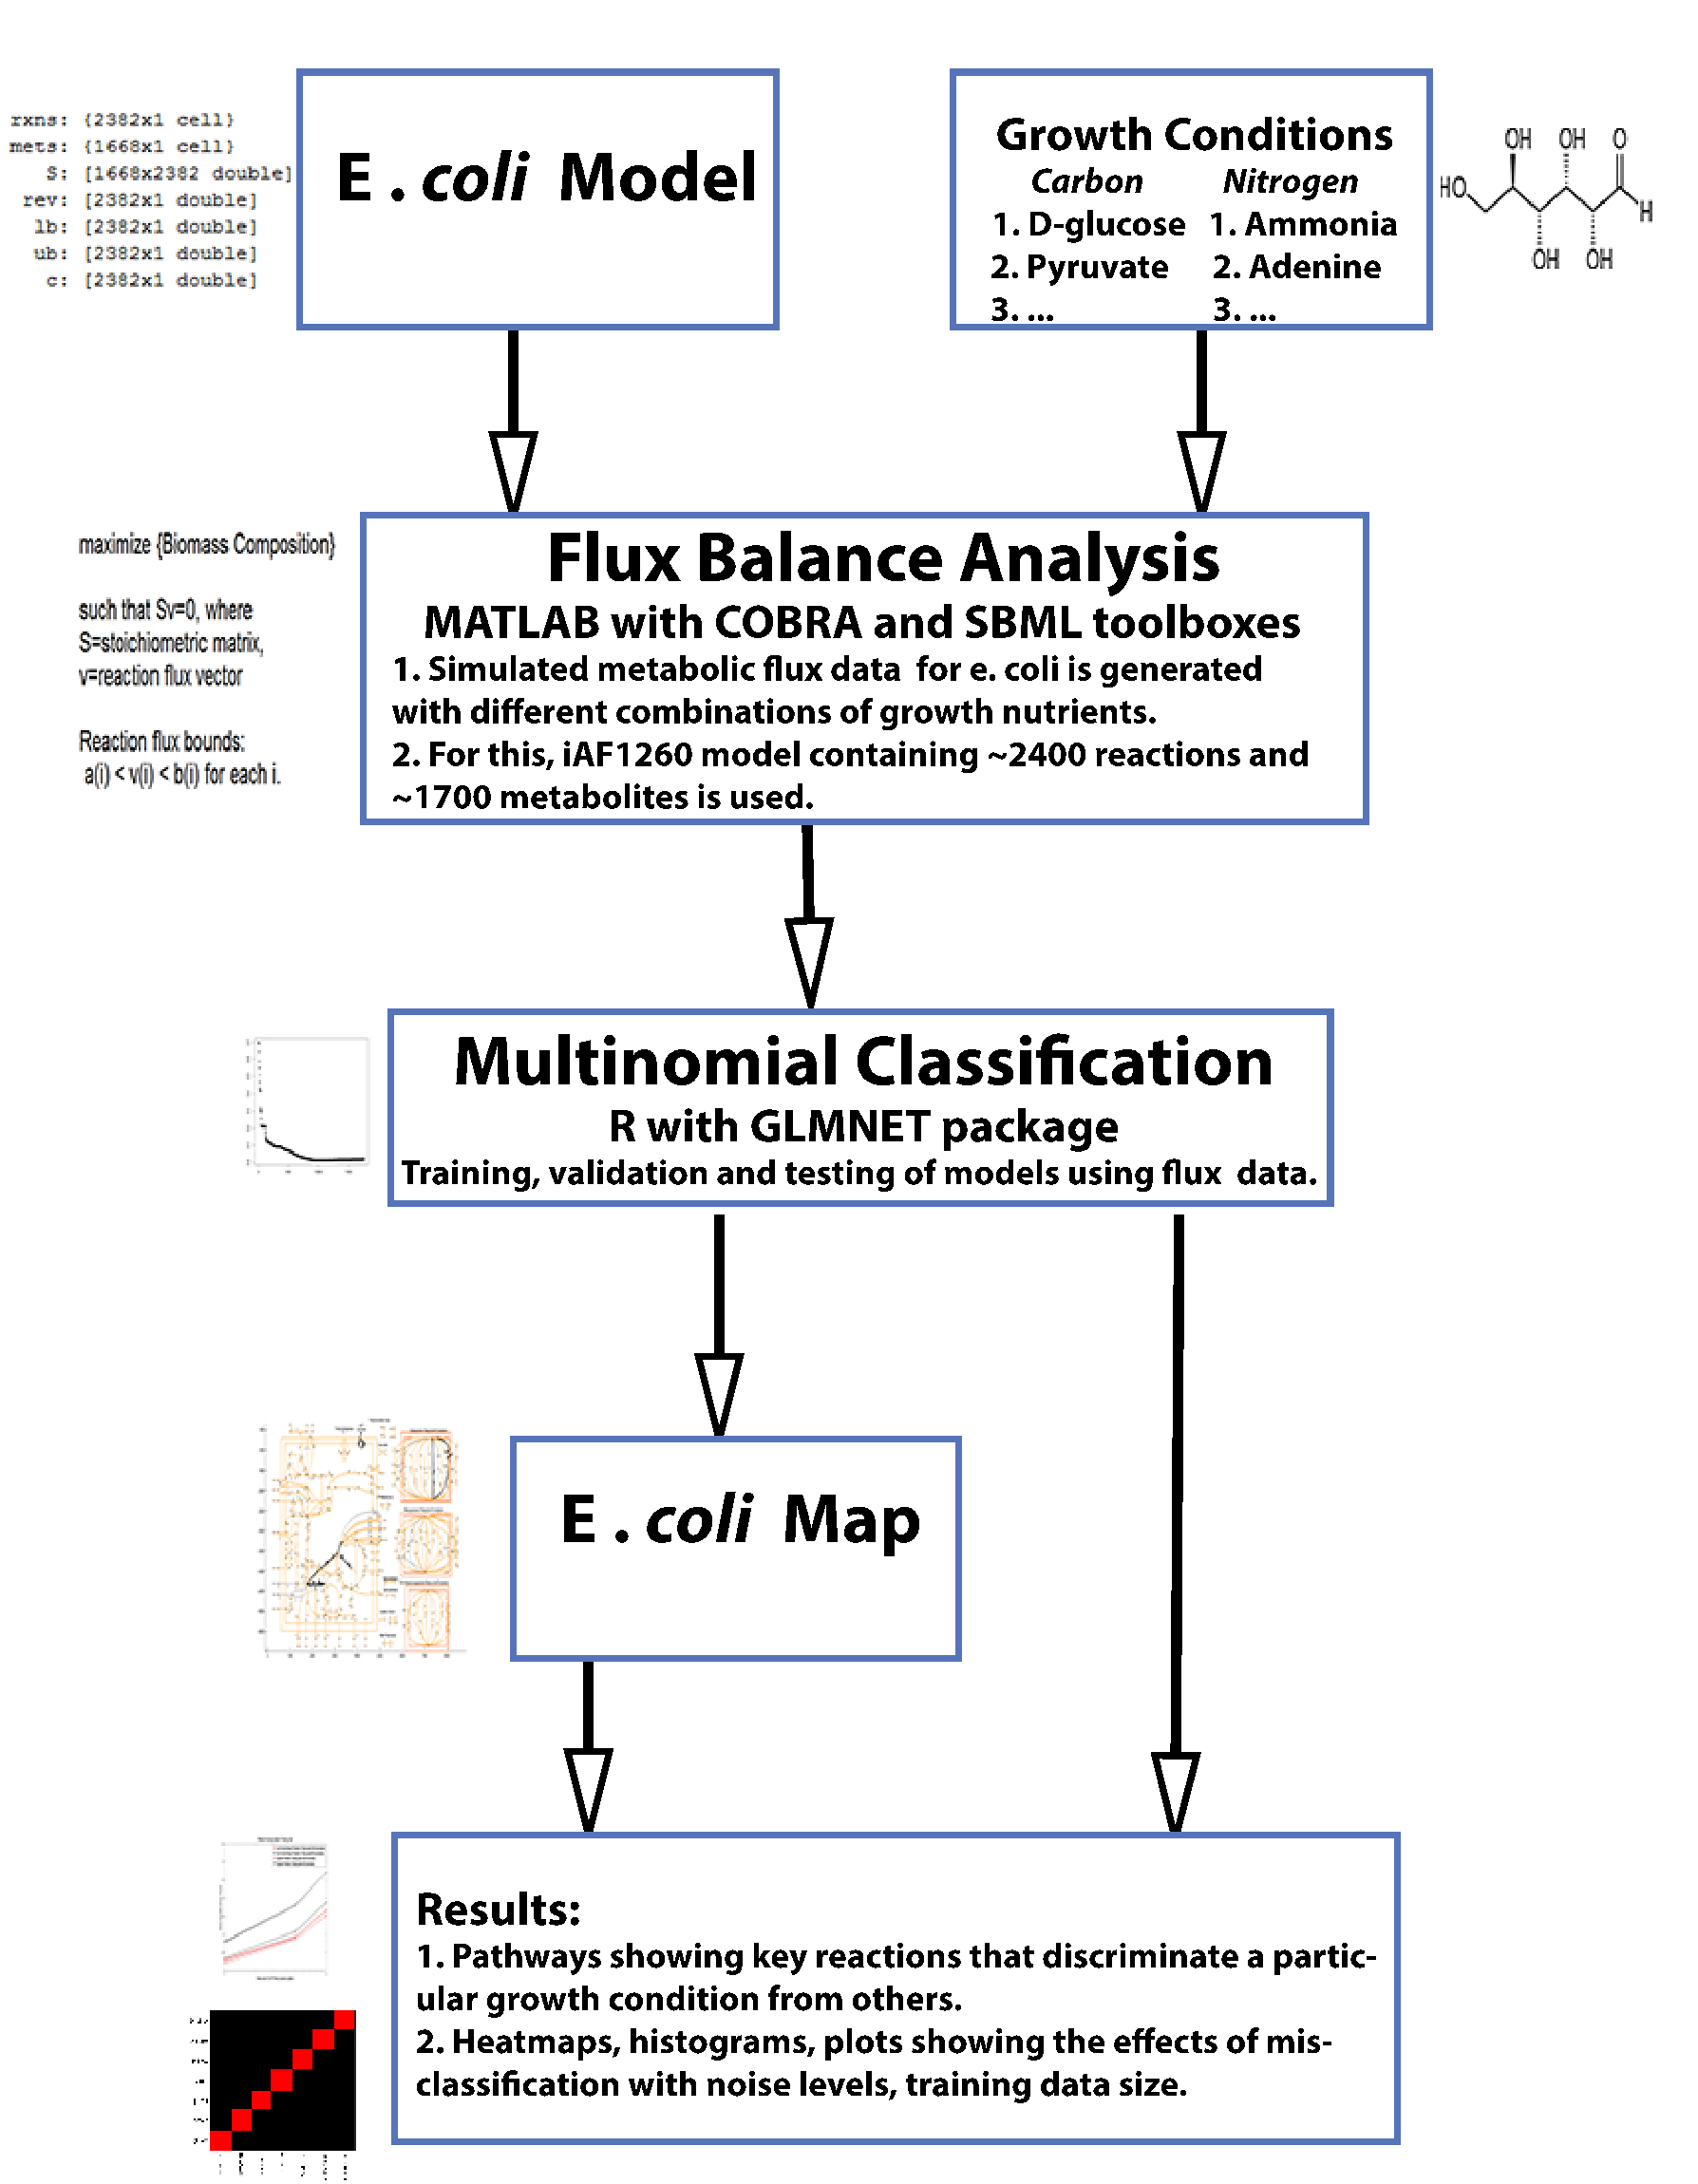
\includegraphics[width=4in]{Figures/flowchart_new.pdf}}
\caption{\label{fig:flowchart}\textbf{Flowchart describing methodology used in this study.} We obtained E. coli model and map from BiGG database. The key steps involved are Flux Balance Analysis and multinomial classification routines.}
\end{figure}

\clearpage
\begin{figure}[!ht]
\centerline{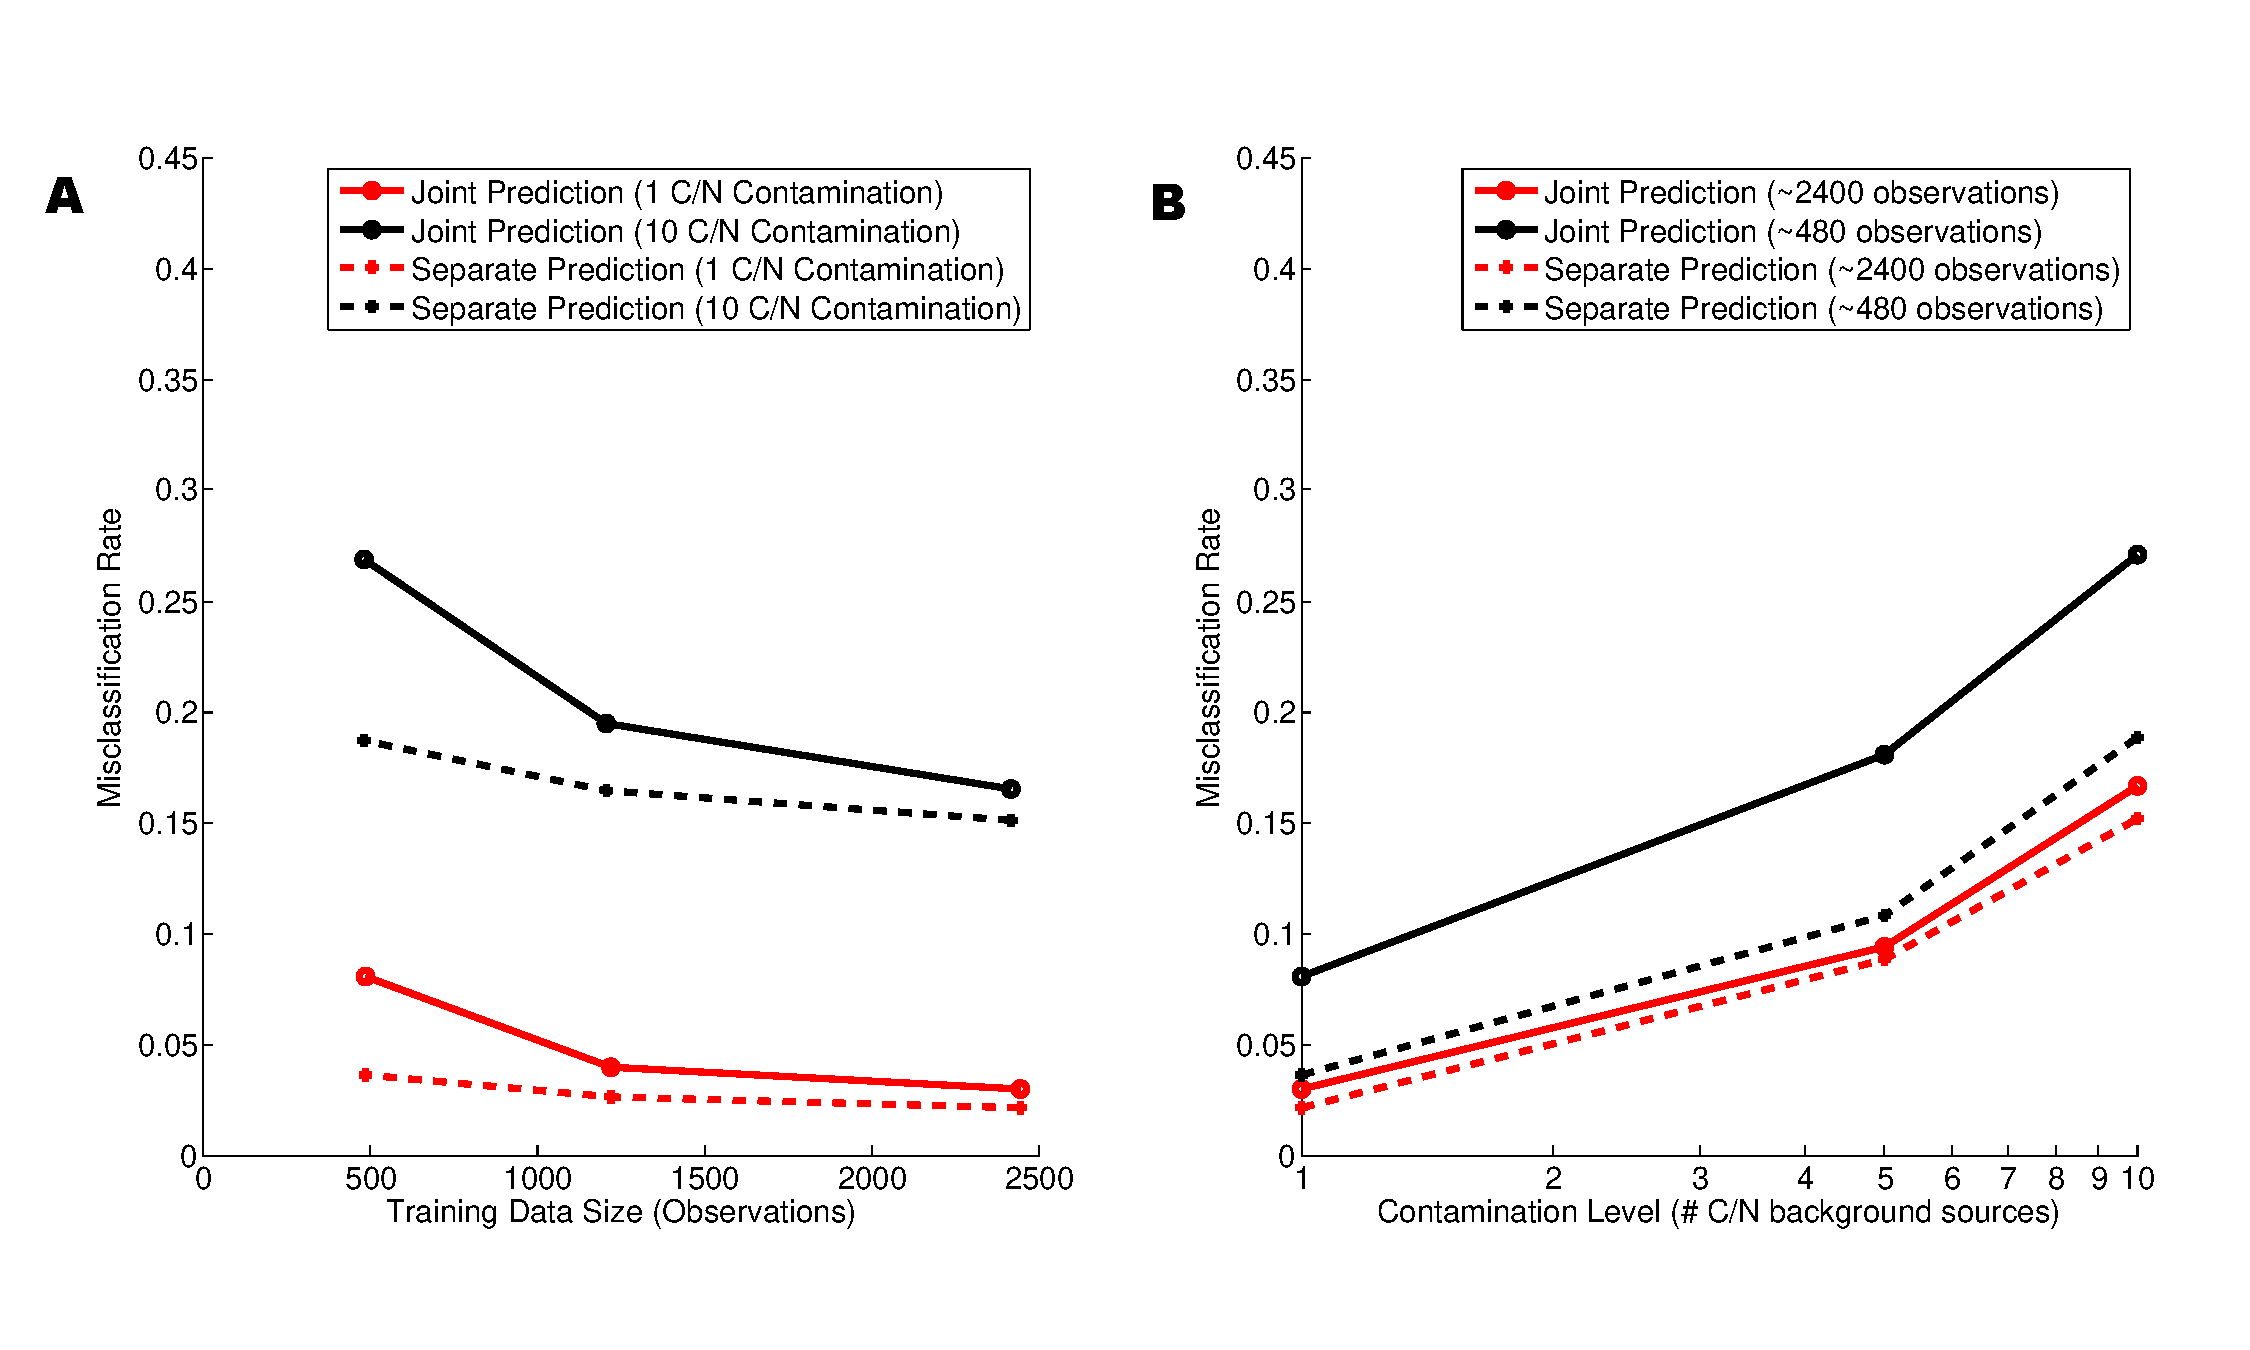
\includegraphics[width=6in]{Figures/combinedContaminationTrainingdata.pdf}}
\caption{\label{fig:misclassification}\textbf{Misclassification rate versus number of contaminants and amount of training data.} (A) The misclassification rate increases as the number of contaminants increases. (B) The misclassification rate decreases as the size of the available training data decreases. In all cases, separate prediction out-performs joint prediction.}
\end{figure}

\clearpage
\begin{figure}[p]
\centerline{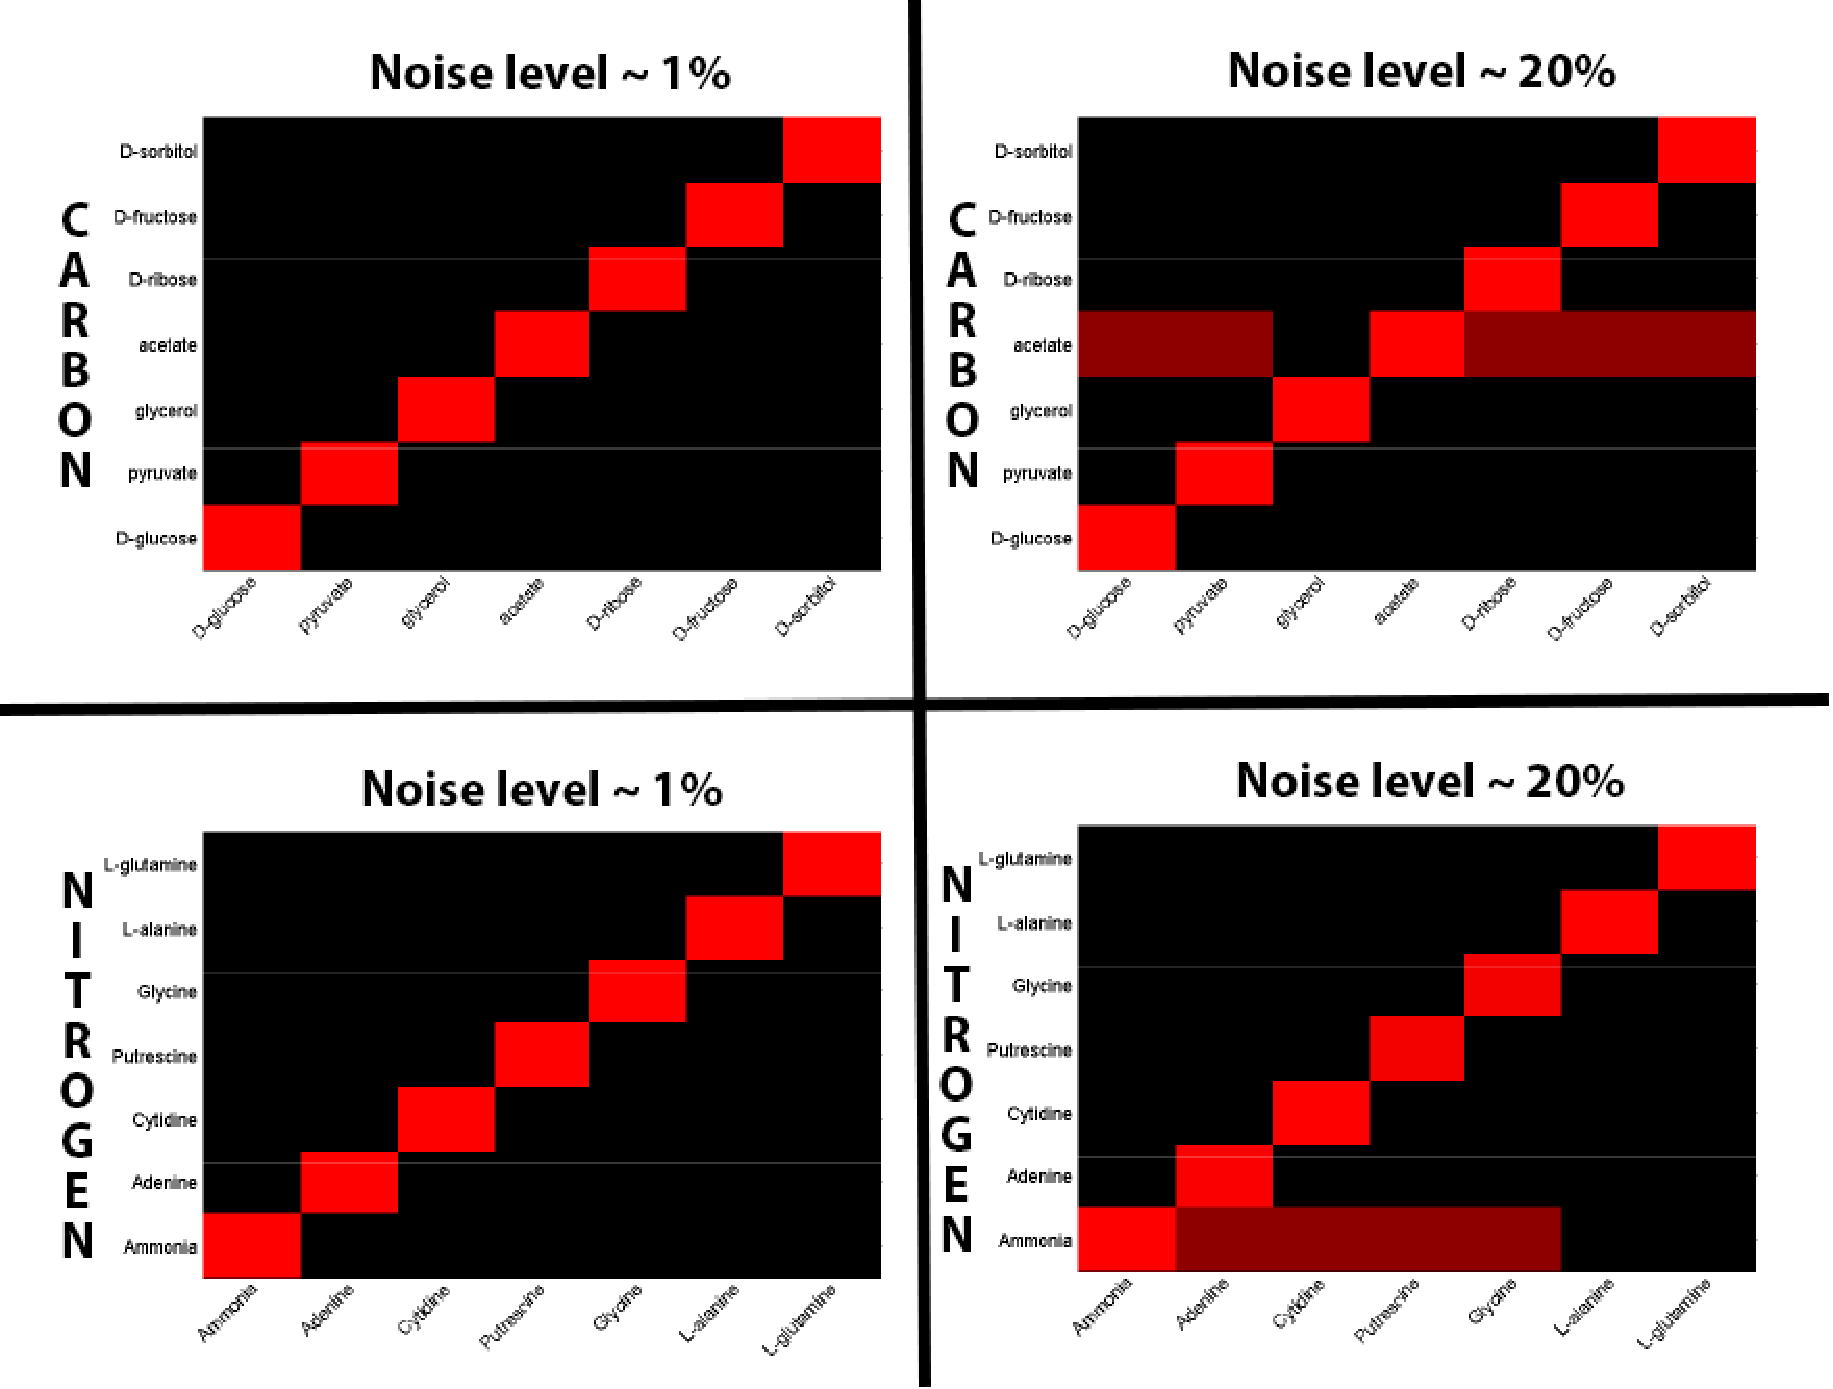
\includegraphics[width=6in]{Figures/heatmap.pdf}}
\caption{\label{fig:heat_map}\textbf{Heat maps with actual sources as columns and predicted ones in rows.}  At 10\% noise, most of the misclassified C sources are predicted wrongly to be acetate and few gets wrongly predicted as pyruvate.}
\end{figure}

\clearpage
\begin{figure}[p]
\centerline{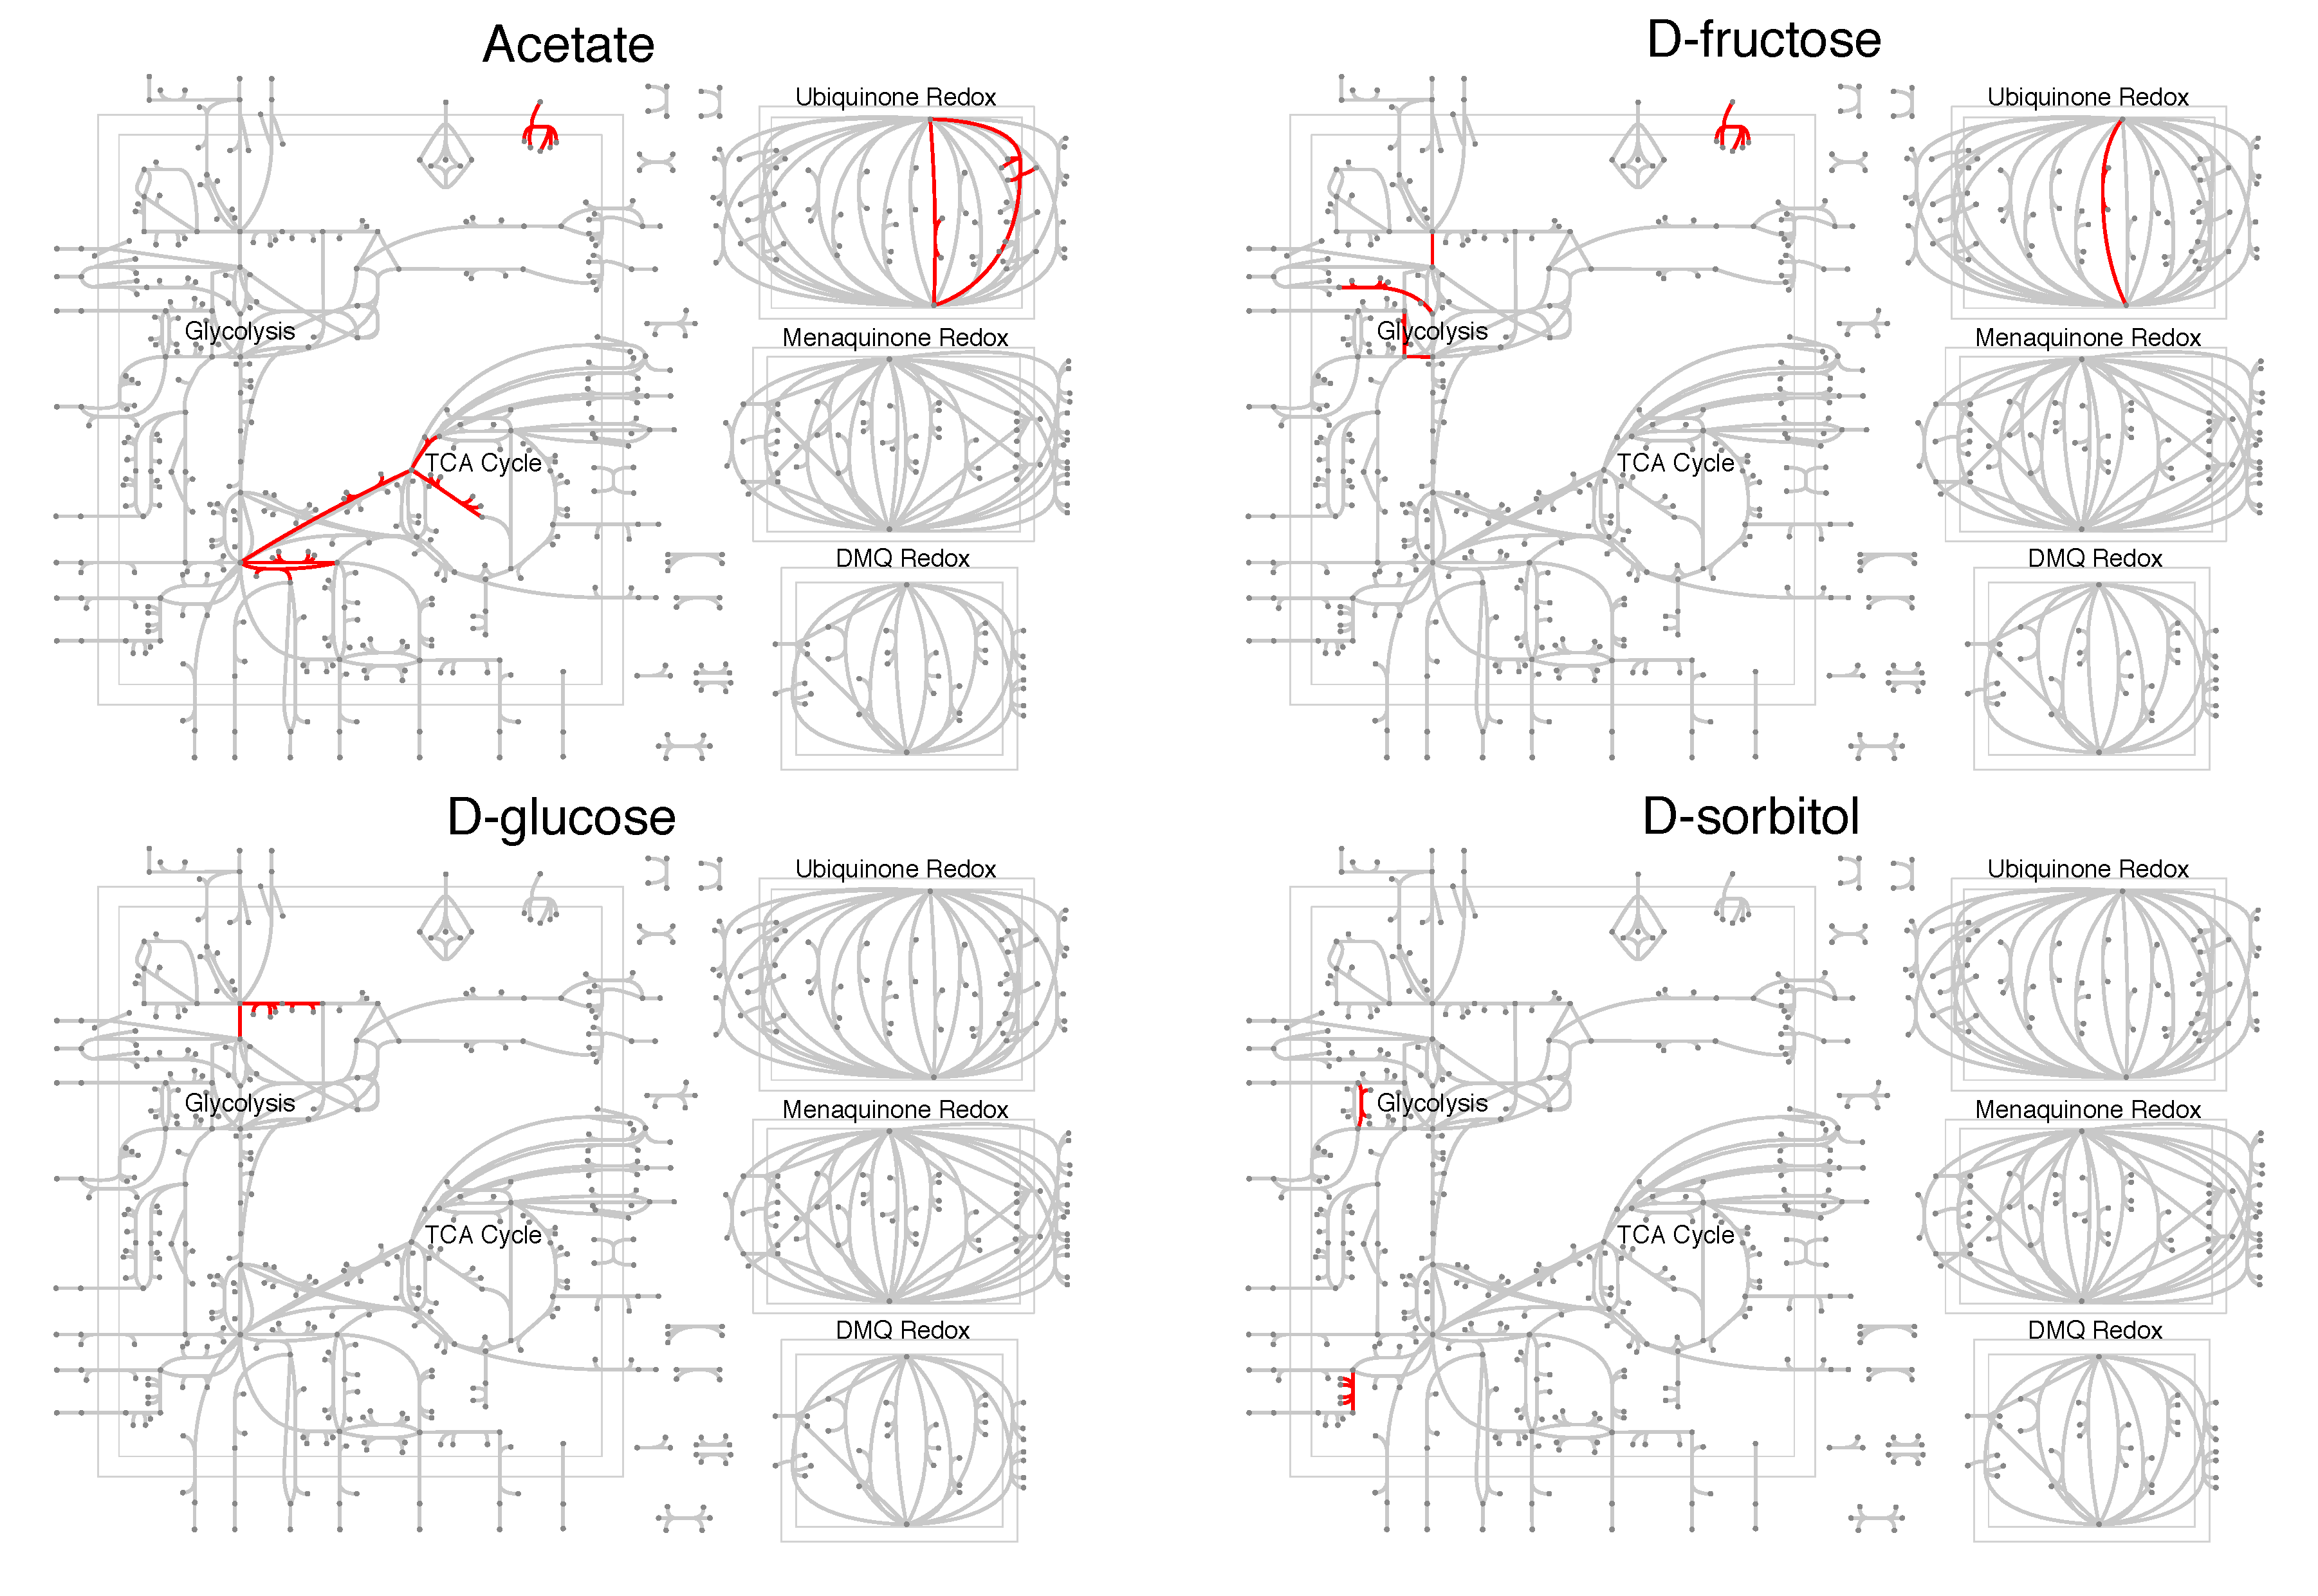
\includegraphics[width=7in]{Figures/carbon/carbon_grid.pdf}}
\caption{\label{fig:carbon_network}\textbf{Discriminatory carbon sources} The key-reactions identified by GLMNET package were mapped onto E. coli central metabolism to visually show the differences between different growth conditions. Out of 7 carbon sources, here we show 4 carbon sources and the key-reactions.}
\end{figure}

\clearpage
\begin{figure}[p]
\centerline{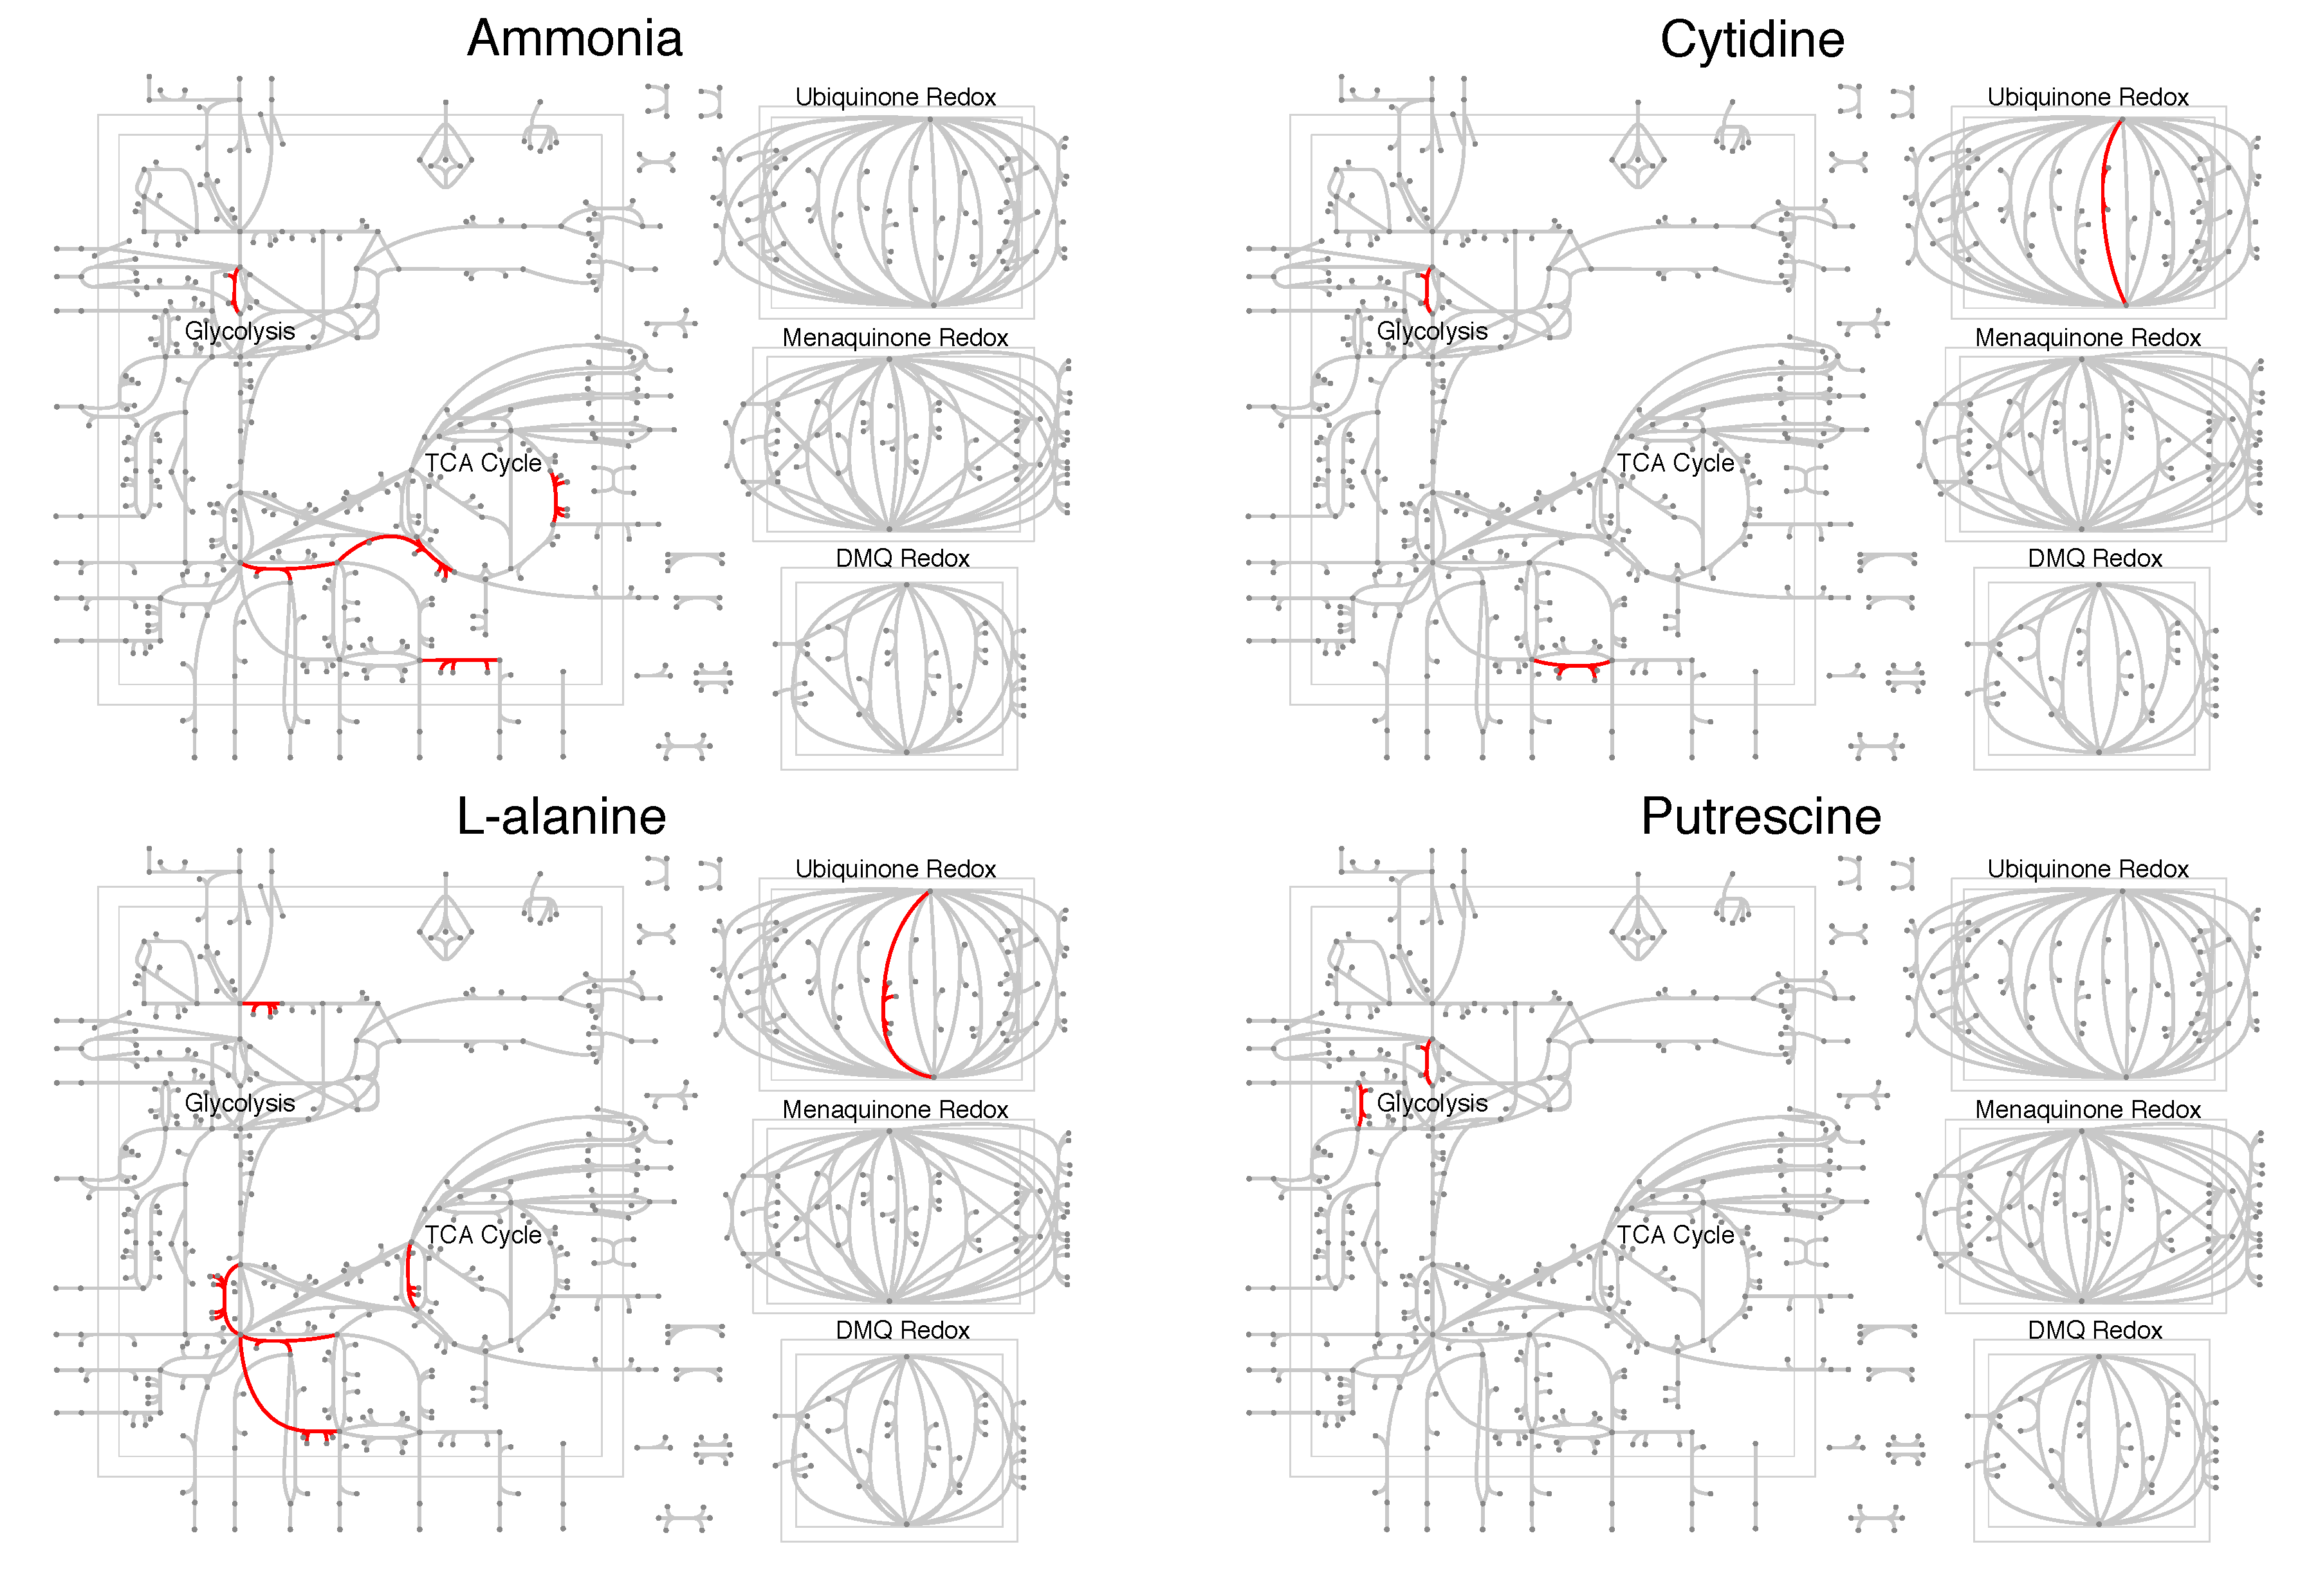
\includegraphics[width=7in]{Figures/nitrogen/nitrogen_grid.pdf}}
\caption{\label{fig:nitrogen_network}\textbf{Discriminatory nitrogen sources} The key-reactions identified by GLMNET package were mapped onto E. coli central metabolism to visually show the differences between different growth conditions. Here, the growth medium used are generally used for K-12 MG1655 strain.}
\end{figure}

\setcounter{figure}{0}
\setcounter{table}{0}

\renewcommand{\figurename}{Supplementary Figure}

\clearpage
\begin{figure}[!ht]
\centerline{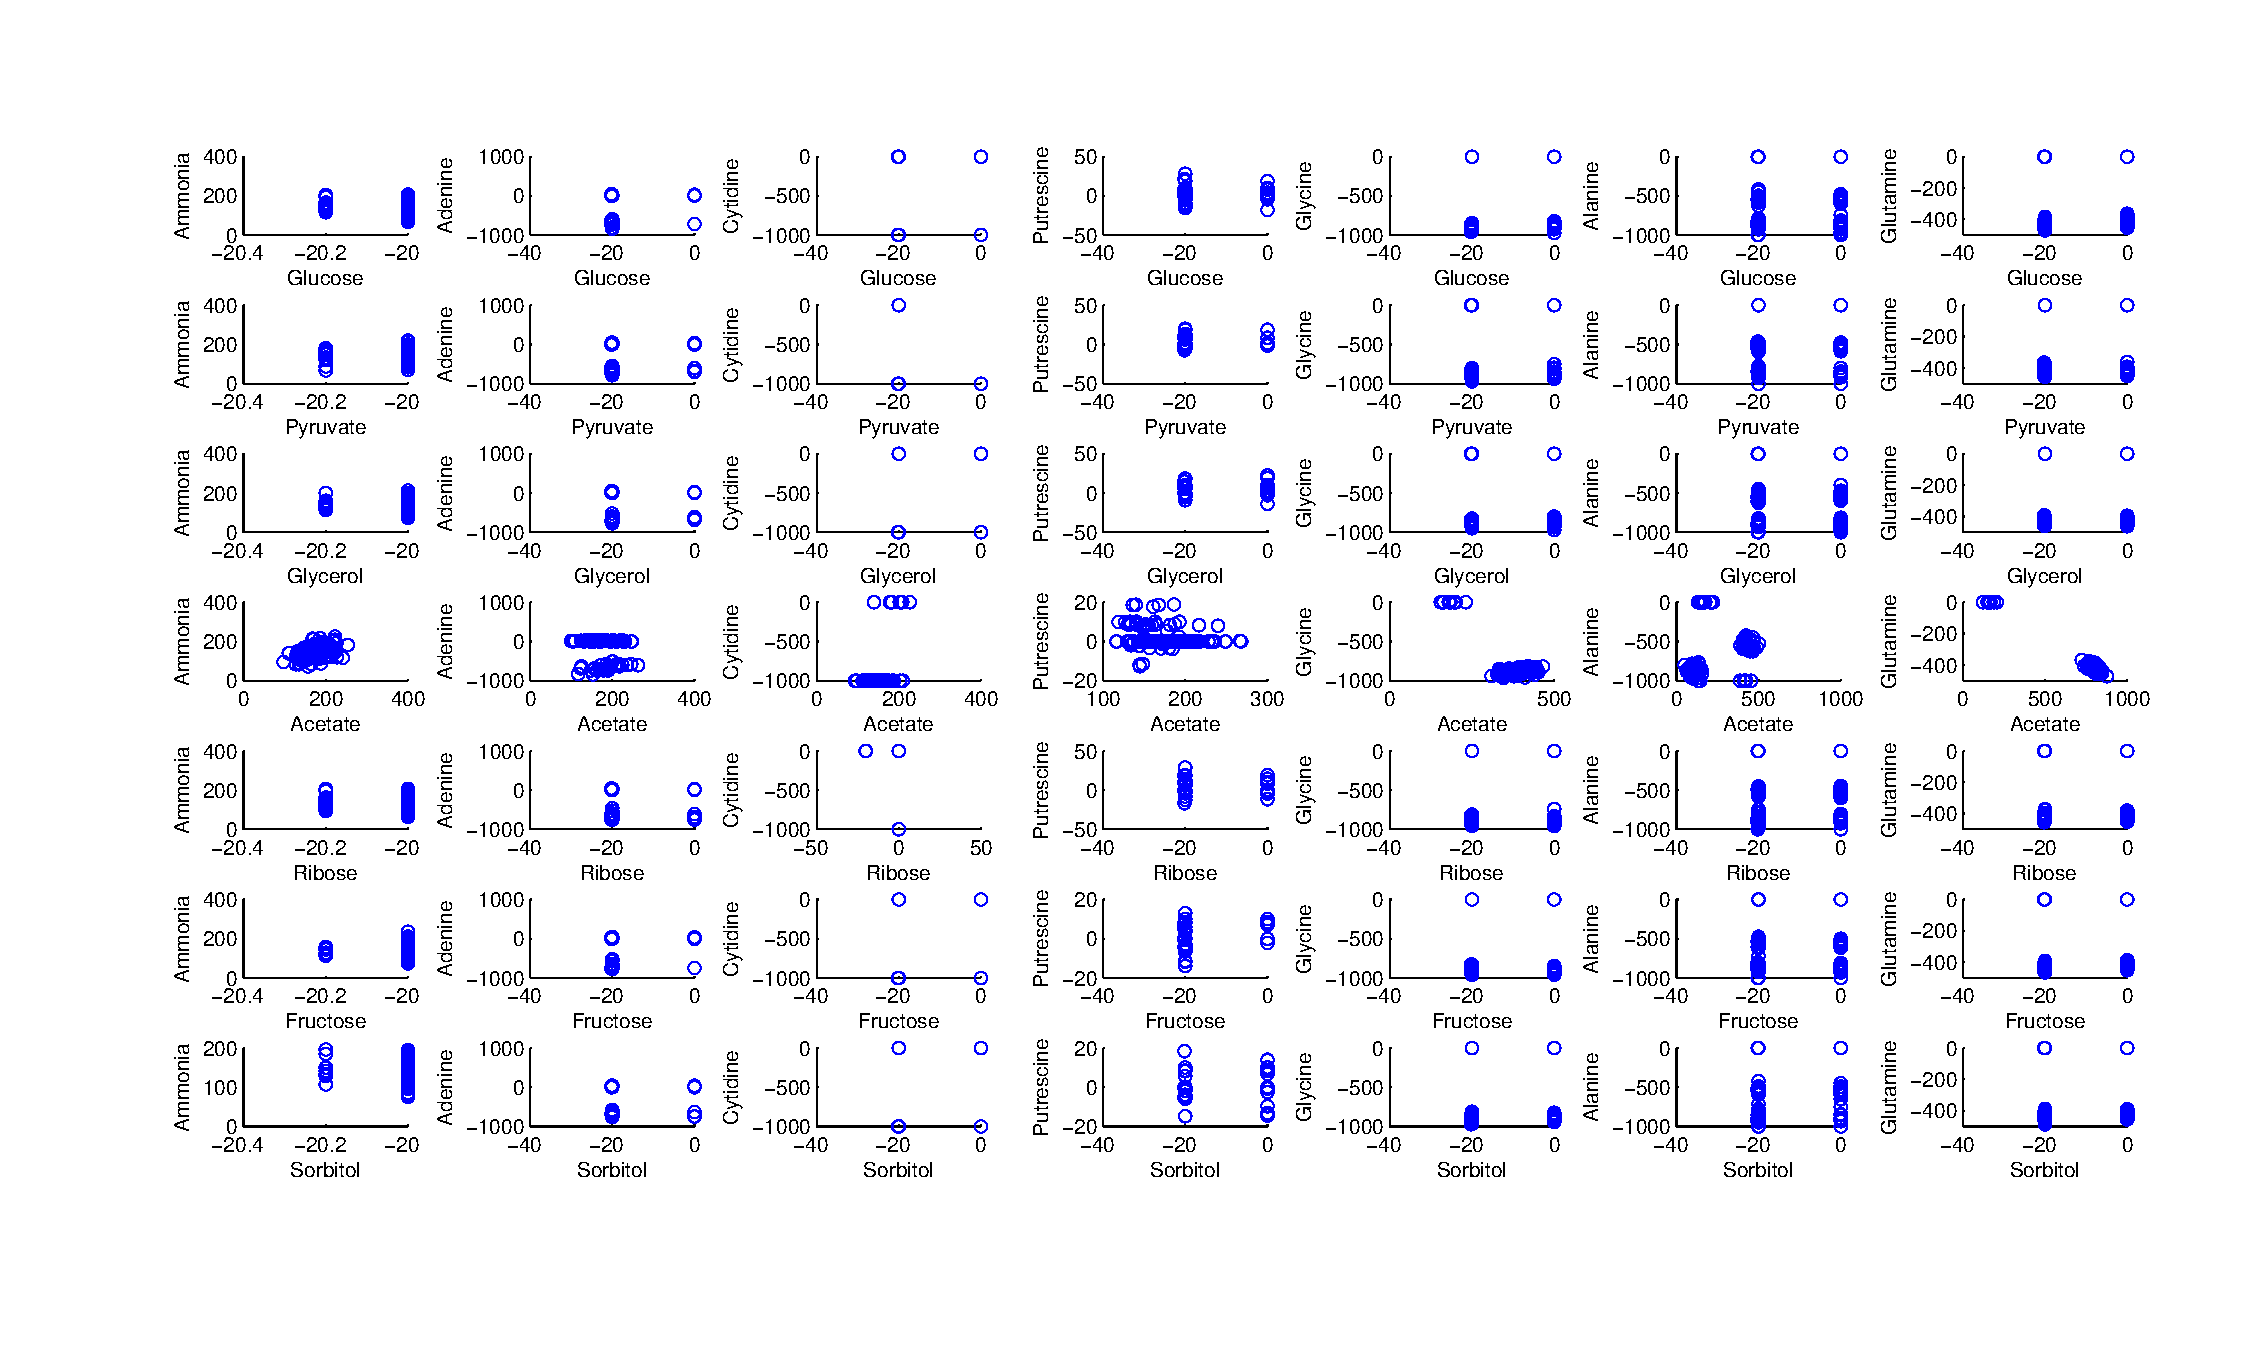
\includegraphics[width=9in]{Figures/SuppInfo/CarbonLimiting.pdf}}
\caption{\label{fig:CarbonLimiting}\textbf{Scatter plot showing varying uptake amounts of C/N sources when carbon source is limited.} We  increased the upper bounds of the nitrogen sources and plotted the uptake amounts of carbon and nitrogen sources.}
\end{figure}

\clearpage
\begin{figure}[!ht]
\centerline{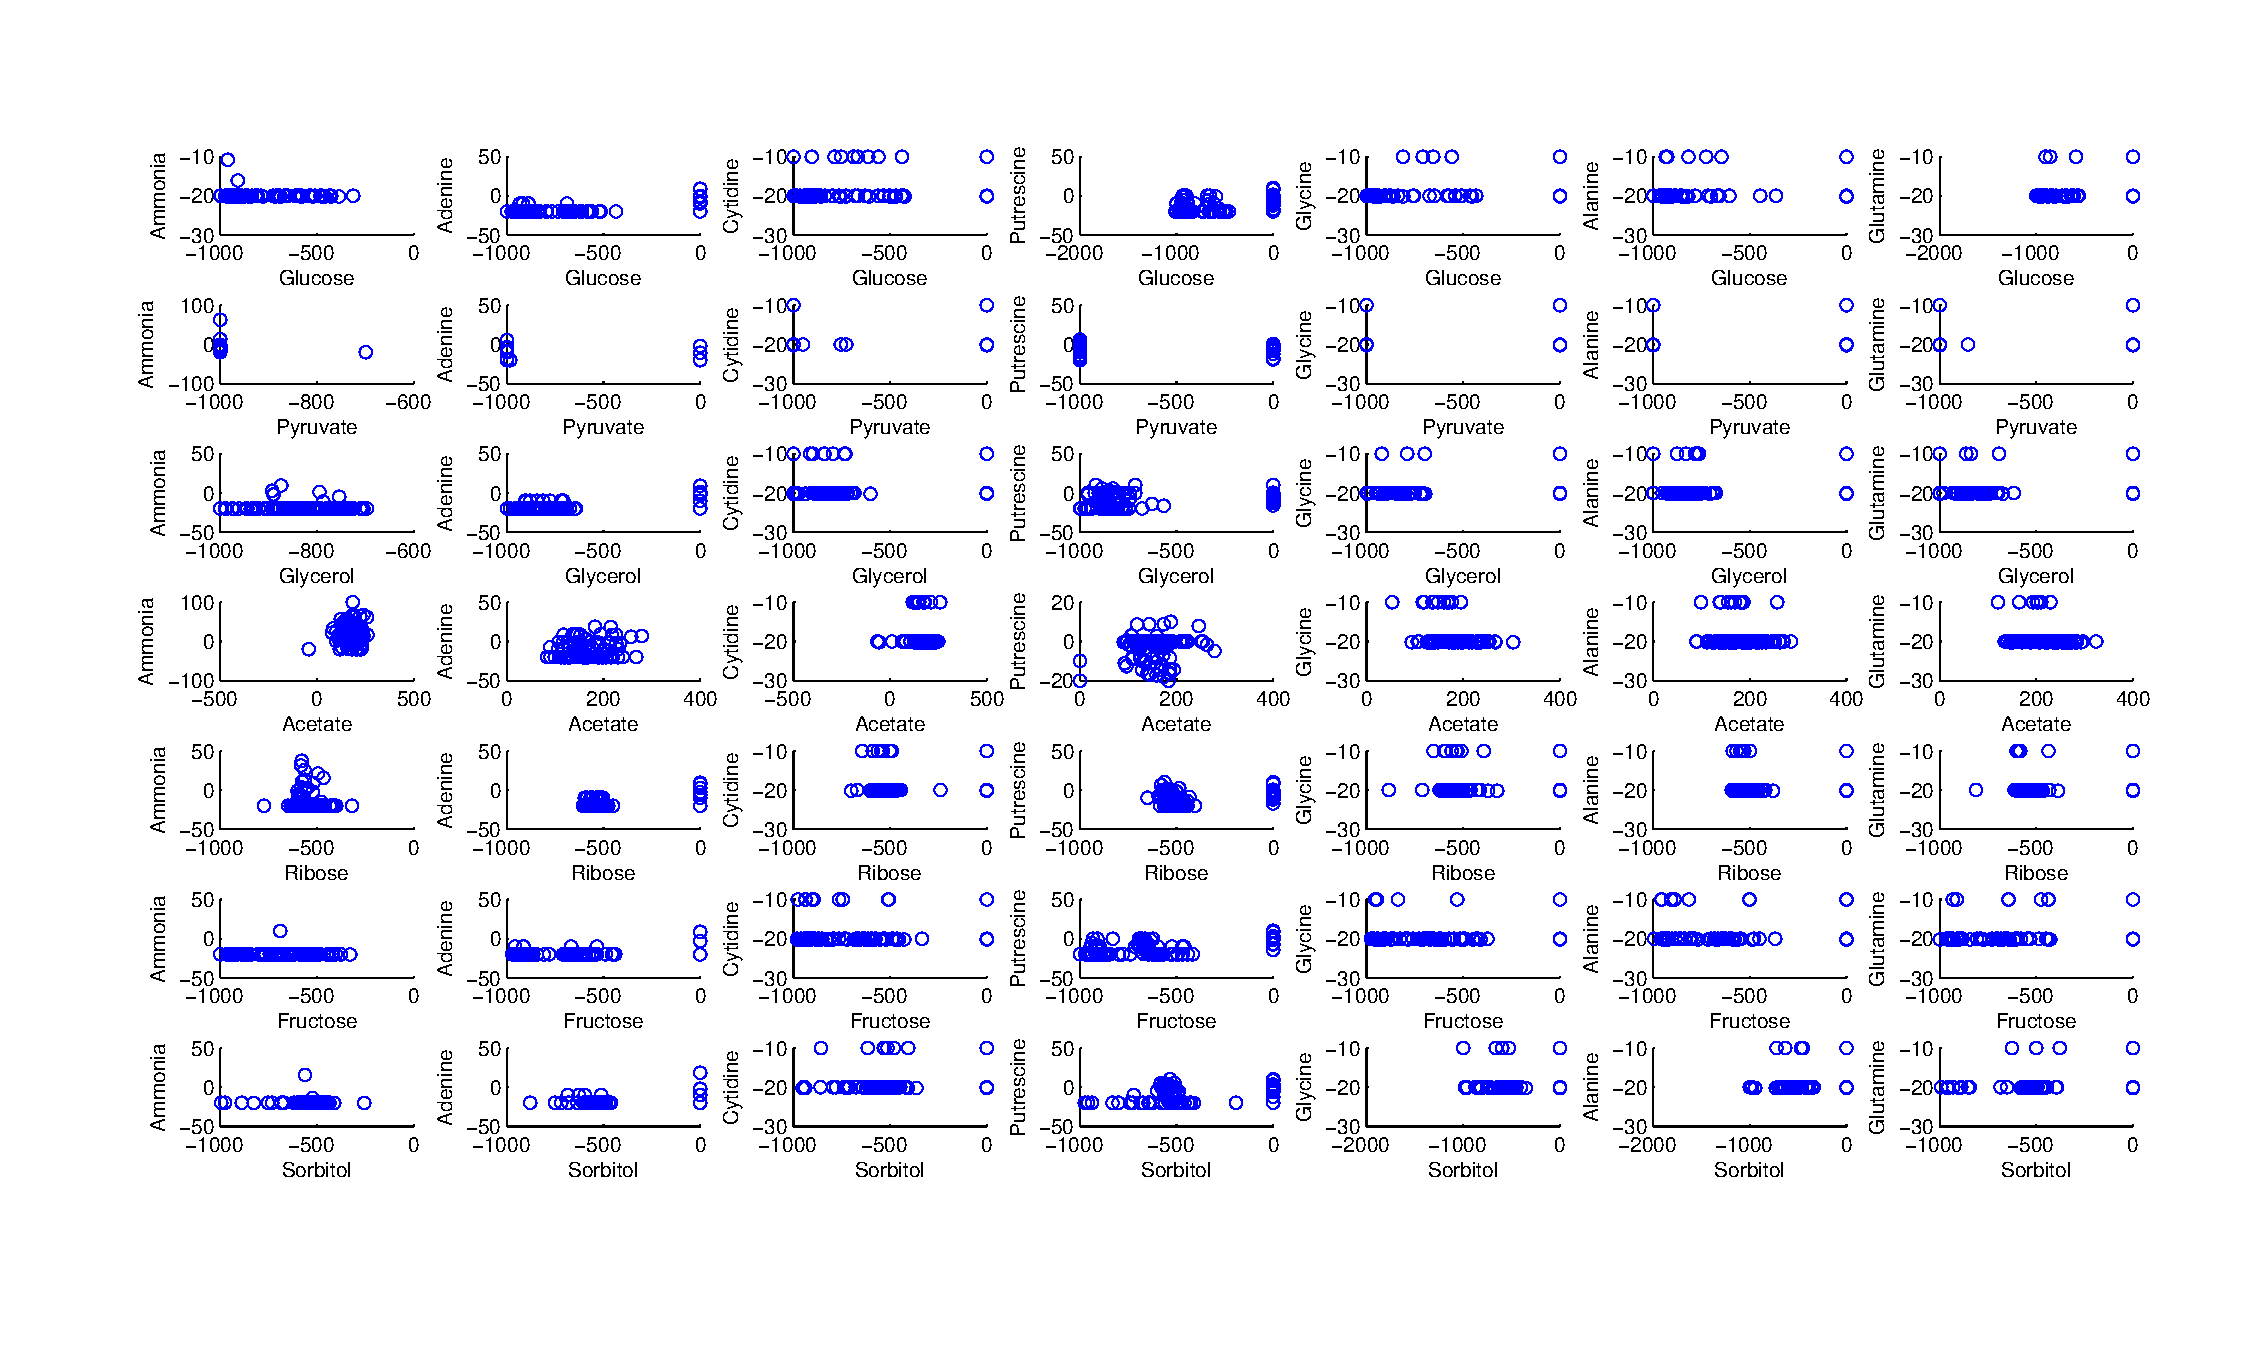
\includegraphics[width=9in]{Figures/SuppInfo/NitrogenLimiting.pdf}}
\caption{\label{fig:NitrogenLimiting}\textbf{Scatter plot showing varying uptake amounts of C/N sources when nitrogen source is limited. }We  increased the upper bounds of the carbon sources and plotted the uptake amounts of carbon and nitrogen sources.}
\end{figure}

\renewcommand{\tablename}{Supplementary Table}

\begin{table}[!ht]
\caption{
\bf{Carbon sources and key reactions identified to discriminate these sources.}}
\end{table}
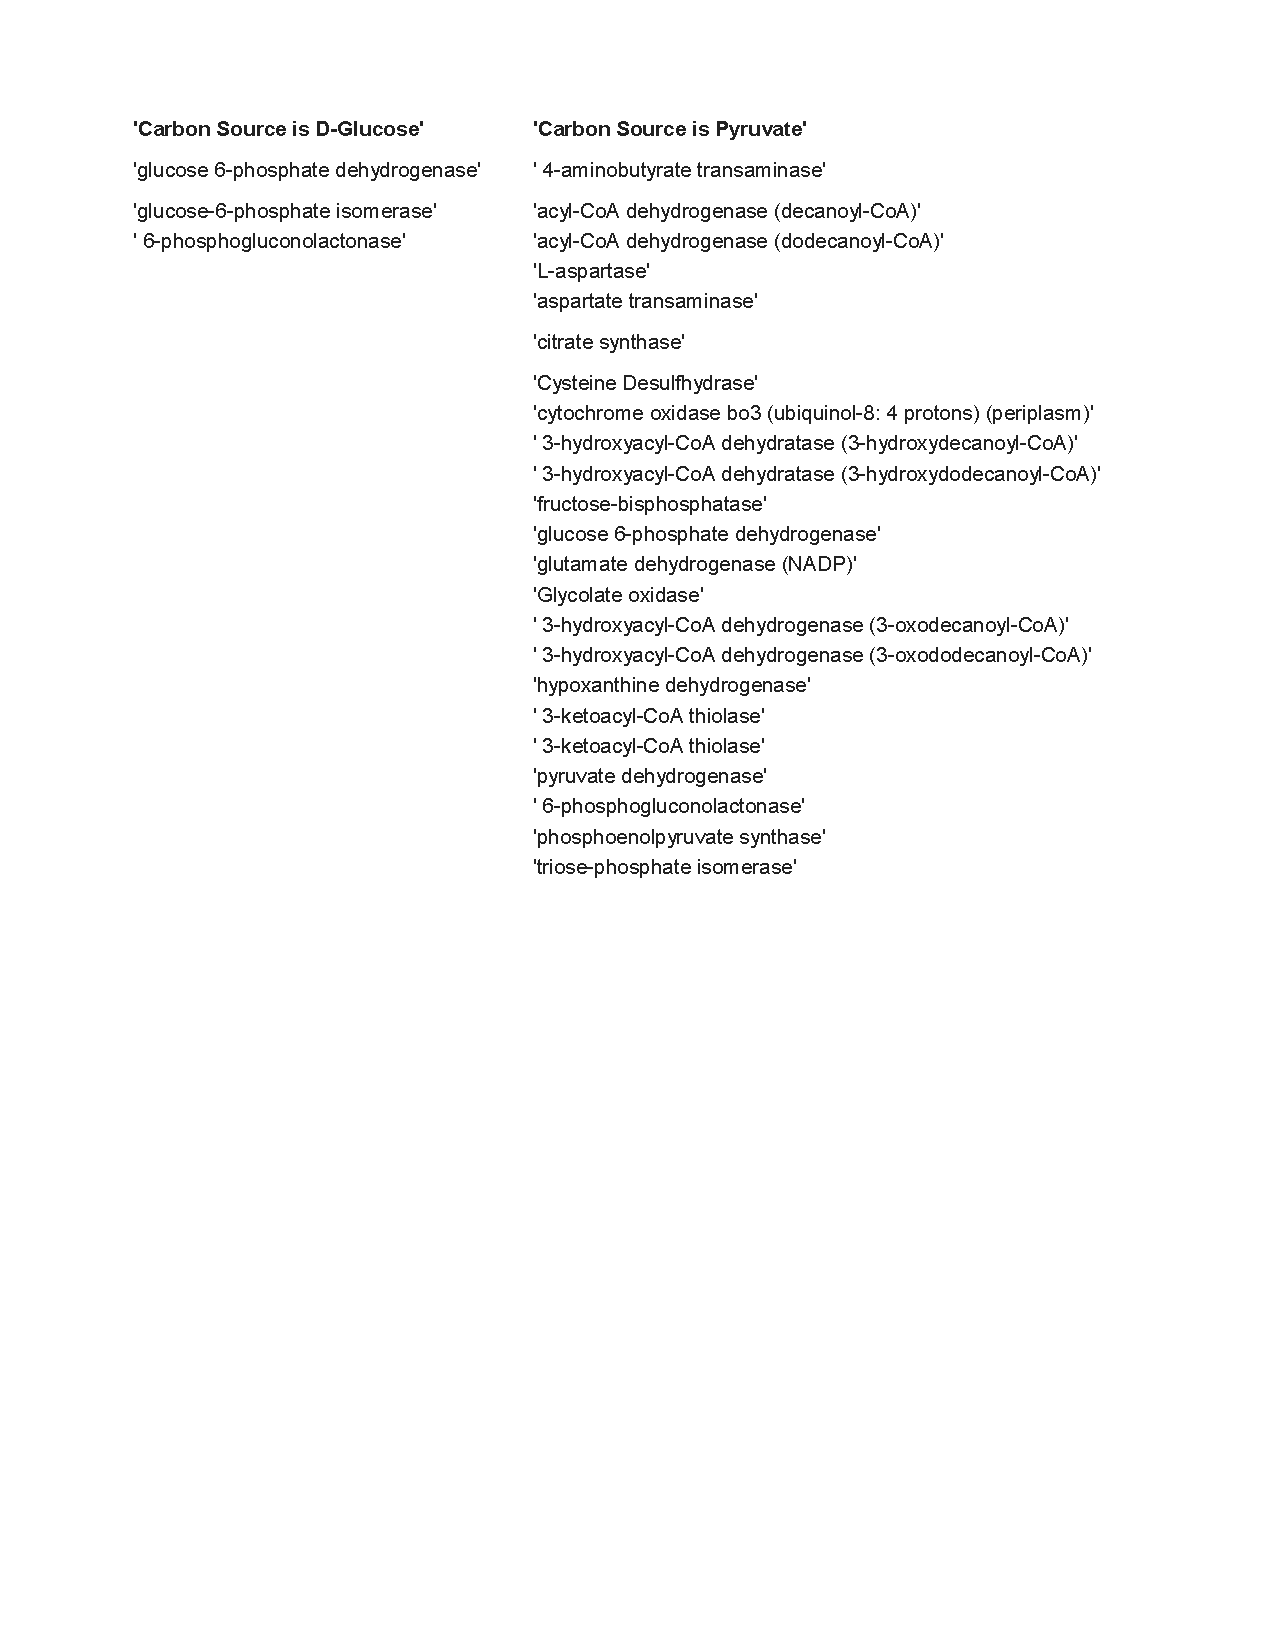
\includegraphics{Figures/SuppInfo/CarbonSources.pdf}
\newpage
\includegraphics[page=2]{Figures/SuppInfo/CarbonSources.pdf}
\newpage
\includegraphics[page=3]{Figures/SuppInfo/CarbonSources.pdf}
\newpage
\includegraphics[page=4]{Figures/SuppInfo/CarbonSources.pdf}
\newpage
\includegraphics[page=5]{Figures/SuppInfo/CarbonSources.pdf}


\begin{table}[!ht]
\caption{
\bf{Nitrogen sources and key reactions identified to discriminate these sources.}}
\end{table}
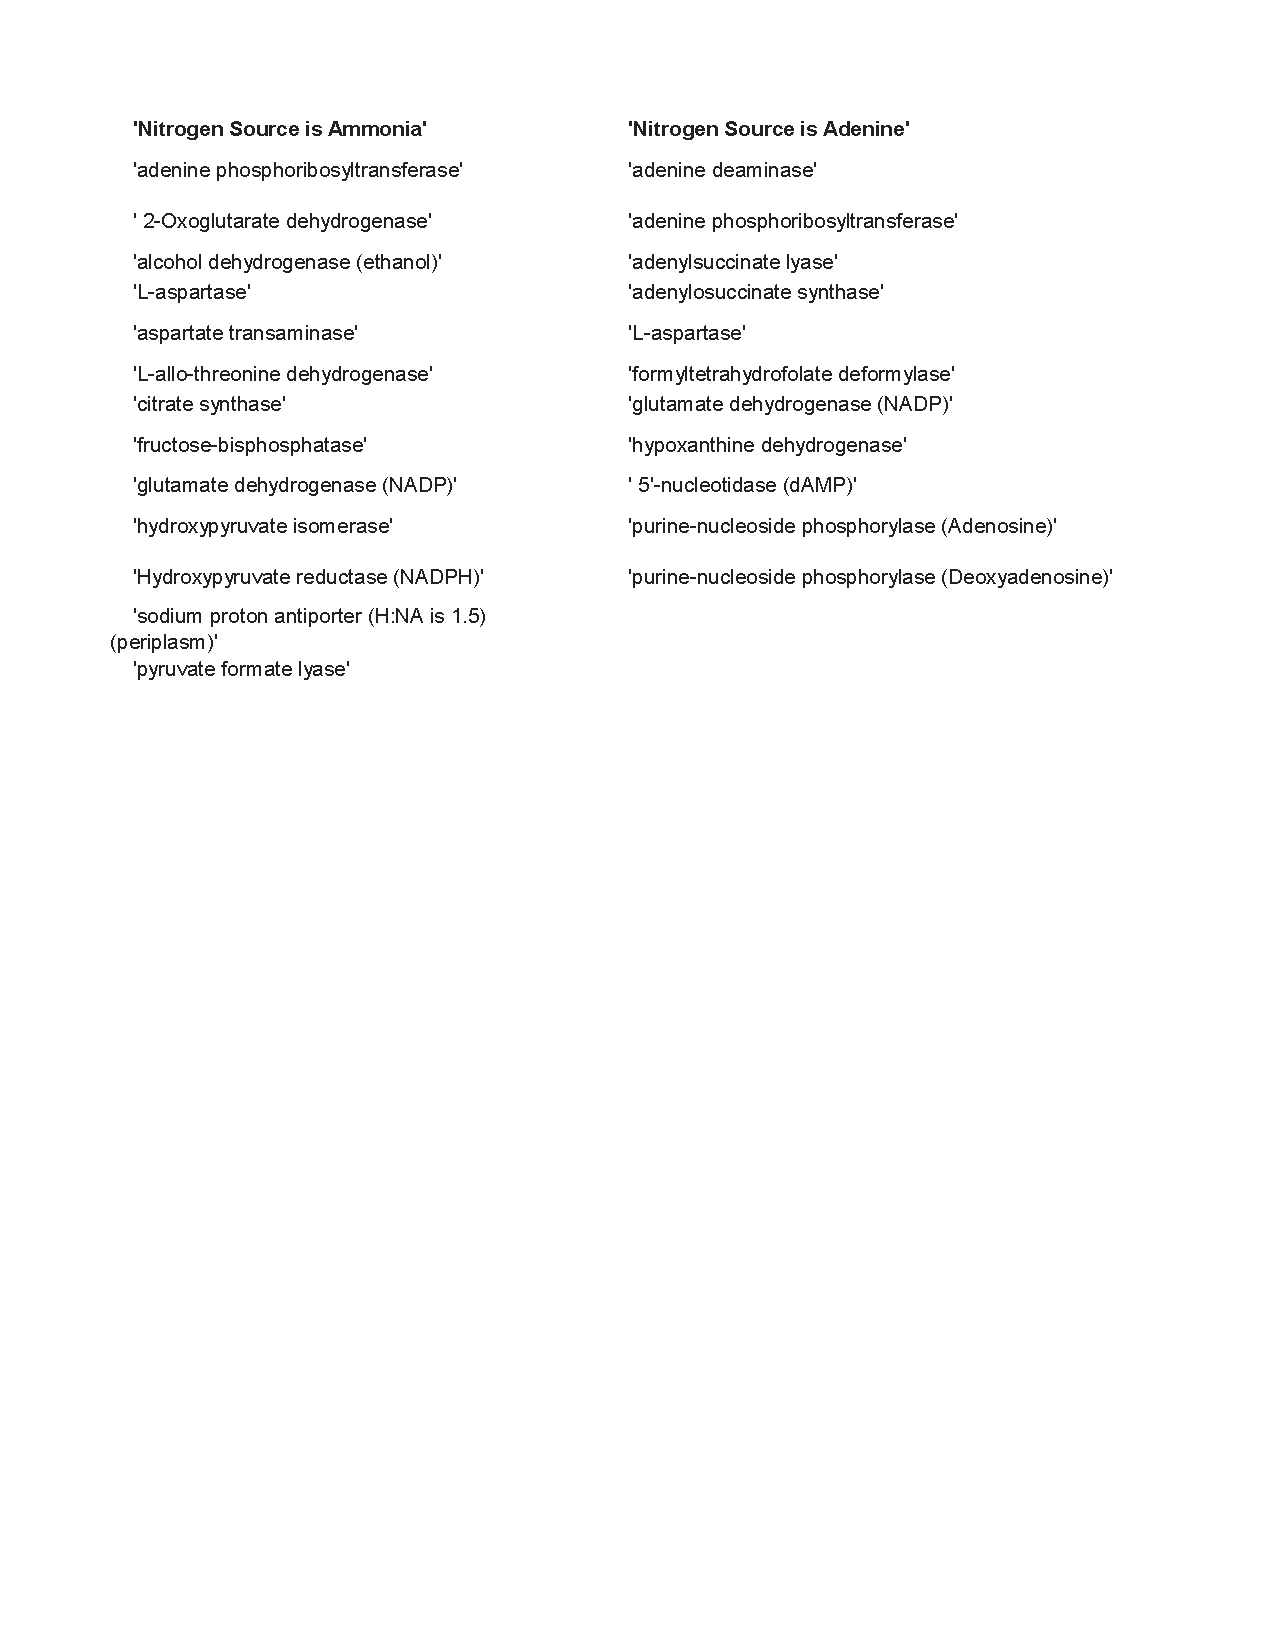
\includegraphics[page=1]{Figures/SuppInfo/NitrogenSources.pdf}
\newpage
\includegraphics[page=2]{Figures/SuppInfo/NitrogenSources.pdf}
\newpage
\includegraphics[page=3]{Figures/SuppInfo/NitrogenSources.pdf}
\newpage
\includegraphics[page=4]{Figures/SuppInfo/NitrogenSources.pdf}


\end{document}


Also, I was thinking would it be helpful to add a line to the contamination/training data size vs misclassification rate plots a line saying "Each data point on joint prediction corresponds to training/testing a new model with LASSO. Similarly for separate prediction, each data point corresponds to training/testing 2 separate models (one each for C and N and then making a joint call)." I don't know if this is important, but I thought I would let you know. So, in that combined plot, in total there were 18 new models trained and tested.
 
Also, the key reactions that were listed in supplementary information were at 1 C/N level and with training data size of ~2450 observations. These reactions were from separately predicting C/N models and hence just represent 1 data point. (I don't know if this should be mentioned in the paper, but I thought to let you know)
 
Also, we used a threshold of 1e-6 on flux measurements to overcome convergence issues. Any flux measurement whose absolute value is less than 1e-6, we rounded off to 0 for LASSO purposes.
